\documentclass{book}
\usepackage[utf8]{inputenc}
\usepackage[T1]{fontenc}
\usepackage{lmodern}
\usepackage[a4paper]{geometry}
\usepackage[frenchb]{babel}
\usepackage{graphicx}
\usepackage{hyperref}

\usepackage{pstricks}
\usepackage{pst-node}
\usepackage{wrapfig}
%\usepackage{picins}
\usepackage{amsmath}


\begin{document}
%%%%%%%%%%%%%%%%%%%%%%%%%%%%%%%%%%%%%%%%%%%%%%%%%%%%%%%%%%%%%%%%%%%%%%%%%%%%%%%%%%%%%%%%%
%=======================================================================================%
%%%%%%%%%%%%%%%%%%%%%%%%%%%%%%%%%%%%%%%%%%%%%%%%%%%%%%%%%%%%%%%%%%%%%%%%%%%%%%%%%%%%%%%%%
\begin{titlepage}
%%%%%%%%%%%%%%%%%%%%%%%%%%  LOGO  %%%%%%%%%%%%%%%%%%%%%%%%%%%%%%%%%%%%%%%%%
 \begin{pspicture}(-5,4)(5,5)
%\rput(-5,3){\href{http://www.upmc.fr/FR/info/00}{
\includegraphics[scale=1.0]{upmc_logo}}}
\rput(-4,6.5){
\includegraphics[scale=1.0]{upmc_logo}}
\rput(-4,5){\resizebox{6cm}{0.3cm}{\begin{tabular}{l}
		Université de Pierre et Marie CURIE (PARIS VI) \\
		4 Place Jussieu 75005 Paris
            \end{tabular}}}
%\psline(-5,0)(5,0)
\end{pspicture}
%%%%%%%%%%%%%%%%%%%%%%%%%%  LOGO  %%%%%%%%%%%%%%%%%%%%%%%%%%%%%%%%%%%%%%%%%
%%%%%%%%%%%%%%%%%%%%%%%%%%  Titre %%%%%%%%%%%%%%%%%%%%%%%%%%%%%%%%%%%%%%%%%
\begin{center}
\resizebox{12cm}{1cm}{\bsc{Priçing d'option financière}}\\
\resizebox{6cm}{0.75cm}{\bsc{par la méthode des EDP}}
\end{center}
%%%%%%%%%%%%%%%%%%%%%%%%%%  Titre  %%%%%%%%%%%%%%%%%%%%%%%%%%%%%%%%%%%%%%%%%
%%%%%%%%%%%%%%%%%%%%%%%%%%  image %%%%%%%%%%%%%%%%%%%%%%%%%%%%%%%%%%%%%%%%%
\begin{pspicture}(-8,-7)(6,8)
%\rput(-5,3){\href{http://www.upmc.fr/FR/info/00}{
\includegraphics[scale=1.0]{upmc_logo}}}
\rput(0,0){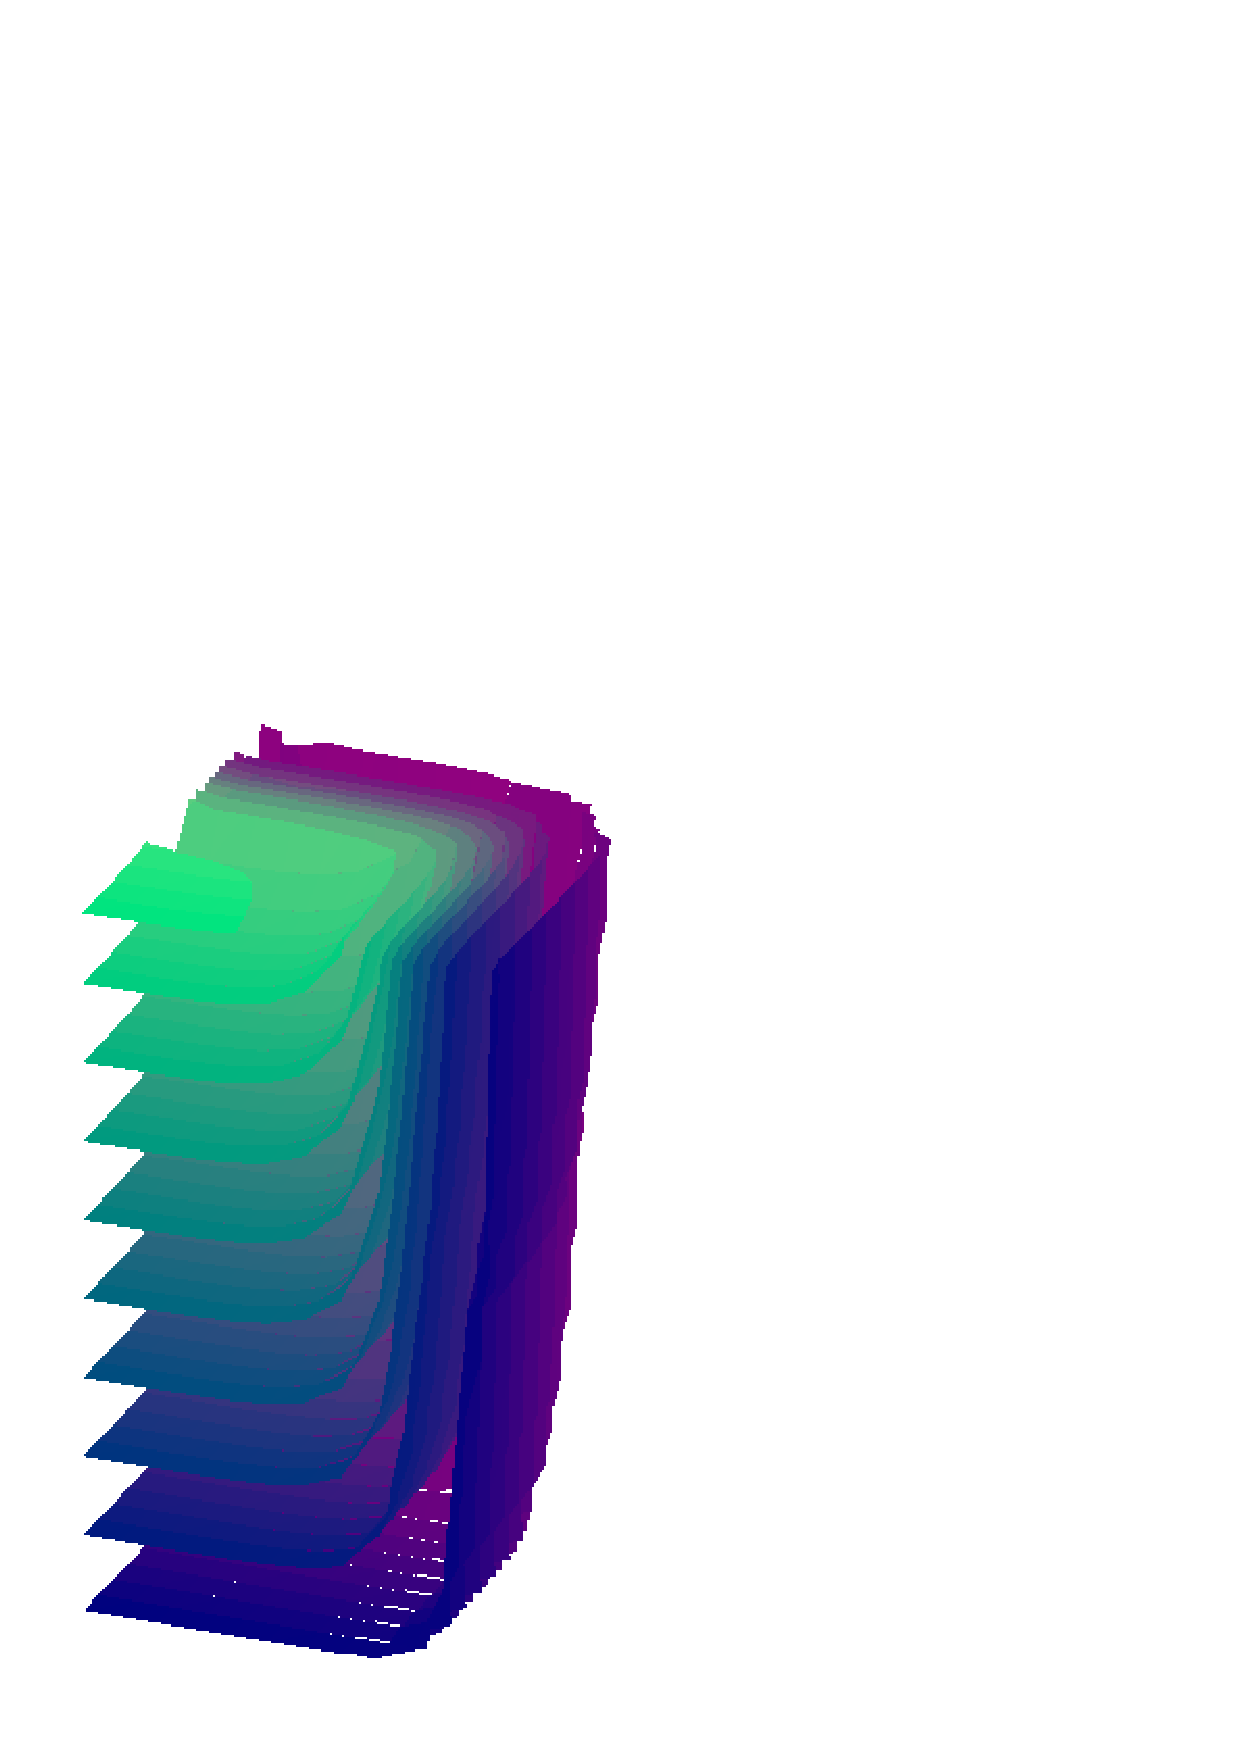
\includegraphics[scale=0.75]{Imagetitle1}}
%\psline(-8,0)(6,0)
\end{pspicture}
%%%%%%%%%%%%%%%%%%%%%%%%%%  image %%%%%%%%%%%%%%%%%%%%%%%%%%%%%%%%%%%%%%%%%
%%%%%%%%%%%%%%%%%%%%%%%%%%  Auteur %%%%%%%%%%%%%%%%%%%%%%%%%%%%%%%%%%%%%%%%%
\begin{flushright}
\underline{\textbf {NGUYEN Chi Thanh}} \\
{\textbf {2007-2008}}
\end{flushright}
%%%%%%%%%%%%%%%%%%%%%%%%%%  Auteur %%%%%%%%%%%%%%%%%%%%%%%%%%%%%%%%%%%%%%%%%


\end{titlepage}
\tableofcontents
%%%%%%%%%%%%%%%%%%%%%%%%%%%%%%%%%%%%%%%%%%%%%%%%%%%%%%%%%%%%%%%%%%%%%%%%%%%%%%%%%%%%%%%%%
%=======================================================================================%
%%%%%%%%%%%%%%%%%%%%%%%%%%%%%%%%%%%%%%%%%%%%%%%%%%%%%%%%%%%%%%%%%%%%%%%%%%%%%%%%%%%%%%%%%
\chapter*{Introduction}
Ce projet est le travail à accomplir pour le module Informatique Scientifique du Master 1 à l'Université Pierre et Marie Curie. Le but essentiel est de calculer la solution des Equations aux Dérivées Partielles par les méthodes numériques, de visualiser la solution par des outils graphiques, en changeant les paramètres de l'équation, on peut voir le comportement de la solution par rapport à l'équation. Les équations résolues dans ce projet sont de type Equations de la chaleur. Plusieurs études mathématiques et informatiques ont été étudiés.
\paragraph{Etudes Mathématiques : } La démonstration d'existance et d'unicité de la solution d'une EDP, des Méthodes de différences finies, Méthodes des éléments finis, Méthodes matricielles comme LU, Gradient Conjugué, GMRES, Méthode de calculer et présenter des iso-surfaces, Méthode de calculer la dérivée par différences finies et différenciation automatique.
\paragraph{Etudes Informatiques : } La programmation C++ pour les calculs scientifiques de haut niveau. La programmation \LaTeX{}, L'initialisation à OpenGL ( Open Graphics Library ), l'utilisation de FreeFem++, GNUplot, Emacs, Linux. 
\paragraph{Le travail : } Il s'agit de calculer la solution des deux équations :
\begin{equation}
\label{equation1}
\partial_{t}u-\frac{\sigma^{2}}{2}\partial_{xx}u-\left(r-\frac{\sigma^{2}}{2}\right)\partial_{x}u+ru=0 
\end{equation}
Le domaine de calcul est : $\Omega \subset R^{2}$ avec $\Omega=\left]-L,L\right[\times\left]O,T\right[$ 
et les conditions aux limites :
\[
\begin{split}
 \hbox{En }t &=0\hbox{,\hspace{0.5cm}} u\left(x,0\right)=\left(K-e^{x}\right)^{+} \\
 \hbox{En }x &=-L\hbox{,\hspace{0.5cm}} u\left(-L,t\right)=Ke^{-rt} \\
 \hbox{En }x &=L\hbox{,\hspace{0.5cm}} u\left(L,t\right)=0
\end{split}
\]
\begin{equation}
\label{equation2}
\frac{\partial u}{\partial t}-\frac{\sigma_{1}^{2}}{2}\frac{\partial^{2}u}{\partial x^{2}}-\frac{\sigma_{2}^{2}}{2}\frac{\partial^{2}u}{\partial y^{2}}-q\sigma_{1}\sigma_{2}\frac{\partial^{2}u}{\partial x\partial y}+\mu_{1}\frac{\partial u}{\partial x}+\mu_{2}\frac{\partial u}{\partial y}+ru=0
\end{equation}
Conditions aux limites :
\begin{itemize}
 \item Conditions Dirichelet : 
	\[u(L,y,t)=u(x,L,t)=0 \hspace{2cm} (x,y)\in \Gamma_{N}\]
 \item Conditions Neumann    : 
	\[\kappa \nabla u.\eta =0 ~~\hbox{sur}\hspace{0.2cm}x=-L~~\hbox{et}\hspace{0.2cm}  y=-L \]
 \item Conditions initiales :
   	\[u(x,y,0)=(K-e^{x}-e^{y})^{+}  \hspace{2cm} (x,y)\in \Omega\] 
\end{itemize}
Les maillages sont d'abord générés avec FreeFem++, puis stoqués dans un fichier numérique. Les données de l'équation sont aussi stoké dans un fichier numérique. Le programme en C++ lit ces fichiers, effectue des calculs afin de sortir une solution sous forme un fichier numérique aussi. La solution peut être visualiser avec l'outil GNUplot. D'un autre côté, l'équation peut être résolue par FreeFem++, puis comparée avec la solution calculée en C++. A la fin, on étend le problème en dimension 3, plus le parametre de fonction qui fait que la solution est de dimension 4. GNUplot ne permet plus à visualiser la solution et fait donc appel à OpenGL, qui utilise la couleur comme le 4ème paramètre. 

Une fois la solution est calculée, quelques tâches supplémentaires sont demandés : Trouver la valeur locale de la solution (sur un point donné), calculer la dérivée de la solution par la méthode de différences finies, et par la méthode de différenciation automatique, puis comparer ces deux résultats.

Le rapport doit être ridigé sous \LaTeX{}. Tout le projet est travailé sous Linux, ainsi que ses outils. 

%%%%%%%%%%%%%%%%%%%%%%%%%%%%%%%%%%%%%%%%%%%%%%%%%%%%%%%%%%%%%%%%%%%%%%%%%%%%%%%%%%%%%%%%%
%=======================================================================================%
%%%%%%%%%%%%%%%%%%%%%%%%%%%%%%%%%%%%%%%%%%%%%%%%%%%%%%%%%%%%%%%%%%%%%%%%%%%%%%%%%%%%%%%%%
\chapter{Projet 1 : Equation de la chaleur}
%%%%%%%%%%%%%%%%%%%%%%%%%%%%%%%%%%%%%%%%%%%%%%%%%%%%%%%%%%%%%%%%%%%%%%%%%%%%%%%%%%%%%%%%%
%=======================================================================================%
%%%%%%%%%%%%%%%%%%%%%%%%%%%%%%%%%%%%%%%%%%%%%%%%%%%%%%%%%%%%%%%%%%%%%%%%%%%%%%%%%%%%%%%%%
\section{Le Problème Mathématique}
%================================================================%
%\subsection{Formule de variationnelle et conditions aux limi&tes}
\paragraph{Equation à résoudre :}
\begin{equation}
\label{énoncé}
\partial_{t}u-\frac{\sigma^{2}}{2}\partial_{xx}u-\left(r-\frac{\sigma^{2}}{2}\right)\partial_{x}u+ru=0
\end{equation}

\paragraph{Conditions aux limites :} 
\begin{wrapfigure}{l}{8cm}
%\parpic{
\centering
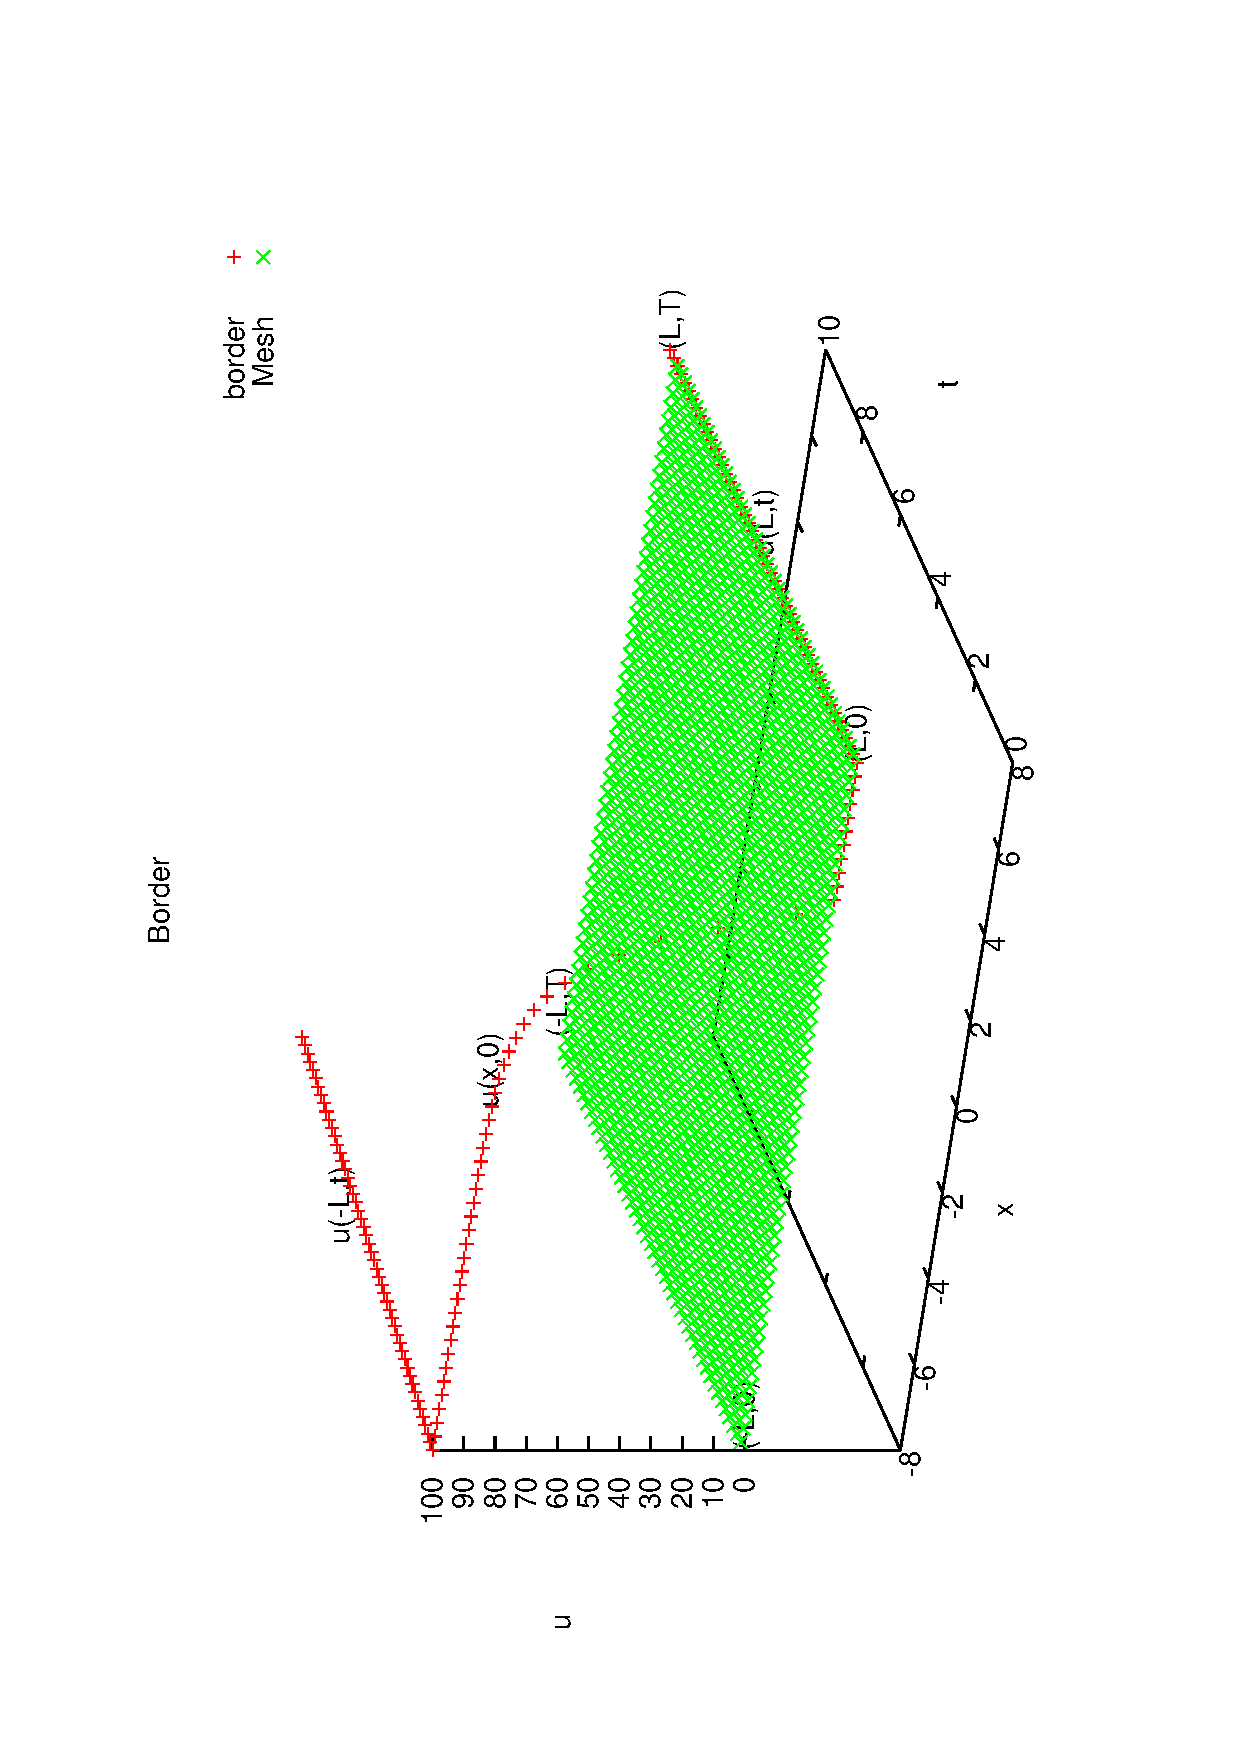
\includegraphics[angle=-90, scale=0.30]{Born}%}
\caption{Border}
\end{wrapfigure} 
$\Omega \in R^{2}$ avec $\Omega=\left]-L,L\right[\times\left]O,T\right[$ 
\vspace{1cm}
\begin{equation}
\label{condition-limite-P1}
%\\ \hbox{Les conditions aux bornes :}
\begin{split}
 \hbox{En }t &=0\hbox{,\hspace{0.5cm}} u\left(x,0\right)=\left(K-e^{x}\right)^{+} \\
 \hbox{En }x &=-L\hbox{,\hspace{0.5cm}} u\left(-L,t\right)=Ke^{-rt} \\
 \hbox{En }x &=L\hbox{,\hspace{0.5cm}} u\left(L,t\right)=0
\end{split}
\end{equation}

\vspace{1.5cm}
\paragraph{Les données}
Il y a 7 constantes données
\begin{itemize}
 \item Les réels $K,L,T,\sigma,r$
 \item Les entiers positif $M,N$ qui sont respectivement le nombre de noeuds en temps $t$ et en $x$
\end{itemize}

%%%%%%%%%%%%%%%%%%%%%%%%%%%%%%%%%%%%%%%%%%%%%%%%%%%%%%%%%%%%%%%%%%%%%%%%%%%%%%%%%%%%%%%%%
%=======================================================================================%
%%%%%%%%%%%%%%%%%%%%%%%%%%%%%%%%%%%%%%%%%%%%%%%%%%%%%%%%%%%%%%%%%%%%%%%%%%%%%%%%%%%%%%%%%
\section{Résolution numérique}
%================================================================%
\subsection{Principes généraux}
Pour la résolution numériquement, il faut en premier discrétiser le domaine de définition. Etant donner $N$ et $M$ qui sont respectivement le nombre des pas de calcul en $x$ et en $t$, on a de différentes manières de discrétisation. Tout dépend de la méthode qui s'appliquera. Nous allons aborder deux maillages différents (qui seront détaillés plus tard) .Ensuite, bien entendu, le but du projet est de trouver la solution de ~\eqref{énoncé}. Supposont que la discrétisation a été faite, $u$ à trouver sera concrètement un tableau de dimension $\left(N+1\right)\times\left(M+1\right)$ . Indexons alors les valeurs à calculer $u_{i}^{j}$ ($i$ et $j$ indexent respectivement $x$ et $t$). Avec les conditions aux limites, nous avons aupparavant $u_{0}^{(j)}$, $u_{N}^{(j)}$,  $u_{(i)}^{0}$ qui sont les conditions aux limites en $x=-L$, $x=L$ et $t=0$. Grâce aux différentes formules d'approximation variationnelles (les schémas numériques), on se ramènes à la résolution d'un système linéaire de la forme :
\begin{equation}
\label{equalineaire}
A.X=B.b
\footnote{pour des raisons de diversités de plusieurs questions en un seul programme, nous insérons la matrice B
dans tous les cas. Même pour le cas non-necessaire, on met $B=I_n$}
\end{equation}
La résolution du système linéaire possède plusieurs méthodes. Nous allons en faire 2 méthodes essentielles et basiques : Méthode directe LU et Méthode itératif Gradient Conjugué, qui seront détaillées plus loin.
%%%%%%%%%%%%%%%%%%%%%%%%%%%%%%%%%%%%%%%%%%%%%%%%%%%%%%%%%%%%%%%%%%%%%%%%%%%%%%%%%%%%%%%%%
%=======================================================================================%
%%%%%%%%%%%%%%%%%%%%%%%%%%%%%%%%%%%%%%%%%%%%%%%%%%%%%%%%%%%%%%%%%%%%%%%%%%%%%%%%%%%%%%%%%
%%%%%%%%%%%%%%%%%%%%%%%%%%%%%%%%%%%%%%%%%%%%%%%%%%%%%%%%%%%%%%%%%%%%%%%%%%%%%%%%%%%%%%%%%
%=======================================================================================%
%%%%%%%%%%%%%%%%%%%%%%%%%%%%%%%%%%%%%%%%%%%%%%%%%%%%%%%%%%%%%%%%%%%%%%%%%%%%%%%%%%%%%%%%%
\section{Les schémas}
%================================================================%
\subsection{Schéma d'Euler implicite}
\[
\label{Euler}
\frac{u_{i}^{j}-u_{i}^{j-1}}{\partial t}-\frac{\sigma^{2}}{2\partial x^{2}}\left[u_{i+1}^{j}-2u_{i}^{j}+u_{i-1}^{j}\right]-\left(\frac{r}{2\partial x}-\frac{\sigma^{2}}{4\partial x}\right)\left[u_{i+1}^{j}-u_{i-1}^{j}\right]+ru_{i}^{j}=0
\]
Par quelques simples calculs : 
\[
u_{i-1}^{j}\left[-\frac{\sigma^{2}}{2\partial x^{2}}+\frac{r}{2\partial x}-\frac{\sigma^{2}}{4\partial x}\right]+u_{i}^{j}\left[\frac{1}{\partial t}+\frac{\sigma^{2}}{\partial x^{2}}+r\right]+u_{i+1}^{j}\left[-\frac{\sigma^{2}}{2\partial x^{2}}-\frac{r}{2\partial x}+\frac{\sigma^{2}}{4\partial x}\right]=\frac{u_{i}^{j-1}}{\partial t}
\]
On est amené donc à la résolution du système linéaire :
\begin{equation}
\left[
\begin{array}{ccccccc}
1\\
a & b & c\\
 & a & b & c\\
 &  & . & . & .\\
 &  &  & a & b & c\\
 &  &  &  & a & b & c\\
 &  &  &  &  &  & 1\end{array}\right]\left[\begin{array}{c}
u_{0}^{j}\\
u_{1}^{j}\\
.\\
.\\
.\\
u_{N-1}^{j}\\
u_{N}^{j}\end{array}\right]=\frac{1}{\partial t}\left[\begin{array}{c}
u_{0}^{j}\\
u_{1}^{j-1}\\
.\\
.\\
.\\
u_{N-1}^{j-1}\\
u_{N}^{j}\end{array}\right]
\hbox{\hspace{2cm}avec, }
\begin{minipage}{5cm}
\flushright
\begin{description}
\item[$a=$]{$\left(-\frac{\sigma^{2}}{2\partial x^{2}}+\frac{r}{2\partial x}-\frac{\sigma^{2}}{4\partial x}\right)$}
\item[$b=$]{$\left(\frac{1}{\partial t}+\frac{\sigma^{2}}{\partial x^{2}}+r\right)$}
\item[$c=$]{$\left(-\frac{\sigma^{2}}{2\partial x^{2}}-\frac{r}{2\partial x}+\frac{\sigma^{2}}{4\partial x}\right)$}
\end{description}
\end{minipage}
\footnote{Les termes aux "bout" du vecteur $u^{j-1}$ doivent s'appliquer pour les conditions aux limites}
\end{equation}
\\ Qui est bien de la forme ~\eqref{equalineaire} : $A.X=B.b$ avec $A$ une matrice tridiagonale, $B=\frac{1}{\partial t}.I_n$, 
\\ La résolution de ce système est décrite dans le paragraphe 4
%================================================================%
\subsection{Schéma de Crank-Nicolson}
\label{Crank}
Rappelons la formule de variationnelle :
\[\partial_{t}u-\frac{\sigma^{2}}{2}\partial_{xx}u-\left(r-\frac{\sigma^{2}}{2}\right)\partial_{x}u+ru=0\]
ou bien :
\[\partial_{t}u=\frac{\sigma^{2}}{2}\partial_{xx}u+\left(r-\frac{\sigma^{2}}{2}\right)\partial_{x}u-ru\]
Par approximation de Crank-Nicolson : 
\[\frac{u^j-u^{j-1}}{\partial t}=\frac{1}{2}.\left(\frac{\sigma^{2}}{2\partial x^{2}}\left[v_{i+1}-2v_{i}+v_{i-1}\right]+\left(\frac{r}{2\partial x}-\frac{\sigma^{2}}{4\partial x}\right)\left[v_{i+1}-v_{i-1}\right]-rv_{i}\right)\]
avec $v=u^{j}+u^{j-1}$. Si on pose encore $w=u^j-u^{j-1}$, on a le système à résoudre : 
\begin{center}
$C.w=D.v$ 
\end{center}
\begin{center}
$C=\frac{1}{\partial t}.I_n$ 
\hbox{, }
$D=\frac{1}{2}.\left[\begin{array}{ccccccc}
1\\
a & b & c\\
 & a & b & c\\
 &  & . & . & .\\
 &  &  & a & b & c\\
 &  &  &  & a & b & c\\
 &  &  &  &  &  & 1\end{array}\right]$ 
\hbox{\hspace{1cm} avec, }
\begin{minipage}{5cm}
\flushright
\begin{description}
\item[$a=$]{$\frac{\sigma^{2}}{2\partial x^{2}}-\frac{r}{2\partial x}+\frac{\sigma^{2}}{4\partial x}$}
\item[$b=$]{$-\frac{\sigma^{2}}{\partial x^{2}}-r$}
\item[$c=$]{$\frac{\sigma^{2}}{2\partial x^{2}}+\frac{r}{2\partial x}+\frac{\sigma^{2}}{4\partial x}$}
\end{description}
\end{minipage}
\end{center}
Ce système est équivalent à $[C-D].u^j=[C+D].u^{j-1}$. En posant $A=[C-D]$, $B=[C+D]$ on revient évidemment au système habituel $A.X=B.b$.
%%%%%%%%%%%%%%%%%%%%%%%%%%%%%%%%%%%%%%%%%%%%%%%%%%%%%%%%%%%%%%%%%%%%%%%%%%%%%%%%%%%%%%%%%
%=======================================================================================%
%%%%%%%%%%%%%%%%%%%%%%%%%%%%%%%%%%%%%%%%%%%%%%%%%%%%%%%%%%%%%%%%%%%%%%%%%%%%%%%%%%%%%%%%%
%%%%%%%%%%%%%%%%%%%%%%%%%%%%%%%%%%%%%%%%%%%%%%%%%%%%%%%%%%%%%%%%%%%%%%%%%%%%%%%%%%%%%%%%%
%=======================================================================================%
%%%%%%%%%%%%%%%%%%%%%%%%%%%%%%%%%%%%%%%%%%%%%%%%%%%%%%%%%%%%%%%%%%%%%%%%%%%%%%%%%%%%%%%%%
\section{Les résolutions du système linéaire}
En reprenant de ce qui précède, on doit résoudre le système de la forme $A.X=B.b$. Mais comme les A, B, b sont données, par un calcul simple de $B.b$ on revient à résoudre un système de la forme $A.X=B$, avec $A$ une matrice tridiagonale. Il ne faut pas oublier dans notre cas, avant l'appel de la résolution du système linéaire, il faut imposer les valeur "au bout" du vecteur $B$ convenable aux conditions de limite.
%================================================================%
\subsection{Méthodes de décomposition LU}
\label{LU}
Soit le système à résoudre : \[A.X=B\footnote{La méthode LU s'applique ssi A est inversible}\]
La méthode de décomposition LU fait parti de la famille de méthodes directes. Le principe est décomposer la matrice A en produit d'une matrice supérieure et une matrice inférieure,puis retrouver la solution en deux étapes par des calculs directs. Donnons dans le cas concret, $A$ est une matrice tridiagonale :
\begin{equation}
\left[\begin{array}{ccccccc}
1\\
a_{2} & b_{2} & c_{2}\\
 & a_{3} & b_{3} & c_{3}\\
 &  & . & . & .\\
 &  &  & a_{n-2} & b_{n-2} & c_{n-2}\\
 &  &  &  & a_{n-1} & b_{n-1} & c_{n-1}\\
 &  &  &  &  &  & 1\end{array}\right]\left[\begin{array}{c}
X_{1}\\
X_{2}\\
.\\
.\\
.\\
X_{n-1}\\
X_{n}\end{array}\right]=\left[\begin{array}{c}
B_{1}\\
B_{2}\\
.\\
.\\
.\\
B_{n-1}\\
B_{n}\end{array}\right]
\end{equation}
Par des calculs de récurrences : \\
\[
\|
	\begin{matrix}
		b_{1}^{*}=b_{1}\\
		c_{1}^{*}=\frac{c_{1}}{b_{1}}
	\end{matrix} \hbox{\hspace{1cm}}
\|
	\begin{matrix}
		b_{j}^{*}=b_{j}-a_{j}.c_{j-1}^{*}\\
		c_{j}^{*}=\frac{c_{j}}{b_{j}^{*}}
	\end{matrix} ,j=1,2...n. \hbox{, en mettant \hspace{0.5cm}}
\|
	\begin{matrix}
		b_{1}=b_{n}=1\\
		a_{1}=a_{n}=c_{1}=c_{n}=0 
	\end{matrix} 
\]

Le système devient $L.U.X=B$ : 
\begin{equation}
\left[\begin{array}{ccccccc}
1\\
a_{2} & b_{2}^{*}  \\
 & a_{3} & b_{3}^{*}  \\
 &  & . & .\\
 &  &  & a_{n-2} & b_{n-2}^{*} \\
 &  &  &  & a_{n-1} & b_{n-1}^{*} \\
 &  &  &  &  &  & 1\end{array}\right].
\left[\begin{array}{ccccccc}
1\\
& 1 & c_{2}^{*}\\
& & 1 & c_{3}^{*}\\
& &  & .  & .\\
& &  &  &  1 & c_{n-2}^{*}\\
& &  &  &  &  1 & c_{n-1}^{*}\\
&  &  &  &  &  & 1\end{array}\right].\left[\begin{array}{c}
X_{1}\\
X_{2}\\
.\\
.\\
.\\
X_{n-1}\\
X_{n}\end{array}\right]=\left[\begin{array}{c}
B_{1}\\
B_{2}\\
.\\
.\\
.\\
B_{n-1}\\
B_{n}\end{array}\right]
\end{equation}

On pose $U.X=Y$, le système se résoud ensuite en deux étapes : 
\[
\begin{split}
\hspace{2cm} L.Y=B \hbox{, se résoud par}
&\Vert \begin{array}{l}
Y_{1}=\frac{B_{1}}{b_{1}^{*}}  \\
Y_{j}=\frac{B_{j}-a_{j}.Y_{j-1}}{b_{j}^{*}}\end{array}
\hbox{\hspace{1cm},} j=2...n 
%\]
\\
%\[
\hspace{2cm} U.X=Y \hbox{, se résoud par}
&\Vert \begin{array}{l}
X_{n}=Y_{n}\\
X_{j}=Y_{j}-c_{j}^{*}.X_{j+1}\end{array}
\hbox{\hspace{1cm},} j=(n-1)...1
\end{split}
\]
%================================================================%
\subsection{Méthodes du Gradient Conjugué}
\label{GC}
Soit le système à résoudre : \[A.X=B\footnote{La méthode du Gradient Conjugué s'applique ssi A est symétrique définie positive}\]
La méthode du Gradient Conjugué fait parti de la famille de méthodes itératives. Le principe est de donner une valeur initiale $x_{0}$, construire la valeur suivante $x_{1}$...et par récurrence, construire une suite $x_{k}$. Et par la théorie mathématique, on démontre que la suite $x_{(k)}$ converge vers la solution cherchée lorsque $k$ tend vers l'infini. La partie théorie mathématique se trouve dans tous les libres de d'analyse numérique matricielle. On expose ici seulement la partie algorithme qui permet de programmer la résolution du système. \\
Soient les valeur données : $A$, $B$, $x_{0}$,$eps$ :
\[
\lVert
\begin{array}{l}
g^{0}=A.x^{0}-B \\
h^{0}=-g^{0} \\
\hbox{Pour }k=0\hbox{ à n} \\
\rho = -\frac{(g^{k},h^{k})}{(h^{k},Ah^{k})} \\
x^{k+1}=x^{k}+\rho h^{k} \\
g^{k+1}=g^{k}+\rho Ah^{k} \\
\gamma = \frac{(g^{k+1},g^{k+1})}{(g^{k},g^{k})}\\
h^{k+1}=-g^{k+1}+\gamma h^{k} \\
\hbox{si }(g^{k+1},g^{k+1}) \leq \epsilon \hbox{ stop}
\end{array}
\]
%%%%%%%%%%%%%%%%%%%%%%%%%%%%%%%%%%%%%%%%%%%%%%%%%%%%%%%%%%%%%%%%%%%%%%%%%%%%%%%%%%%%%%%%%
%=======================================================================================%
%%%%%%%%%%%%%%%%%%%%%%%%%%%%%%%%%%%%%%%%%%%%%%%%%%%%%%%%%%%%%%%%%%%%%%%%%%%%%%%%%%%%%%%%%
\section{Maillage}
Nous n'abordons ici que des maillages rectangulaires, ce qui fait que les paramètres $x$ et $t$ seront distribués indépendemment. Pour la première étape, on distribue les points régulièrement (FiG-gauche). Ensuite, pour une demande de précision autour d'un point ($x=Log(K)$) , on distribue les points par méthode dite dictonomie (FiG-droite).  

\paragraph{Les Maillages}
\begin{center}
 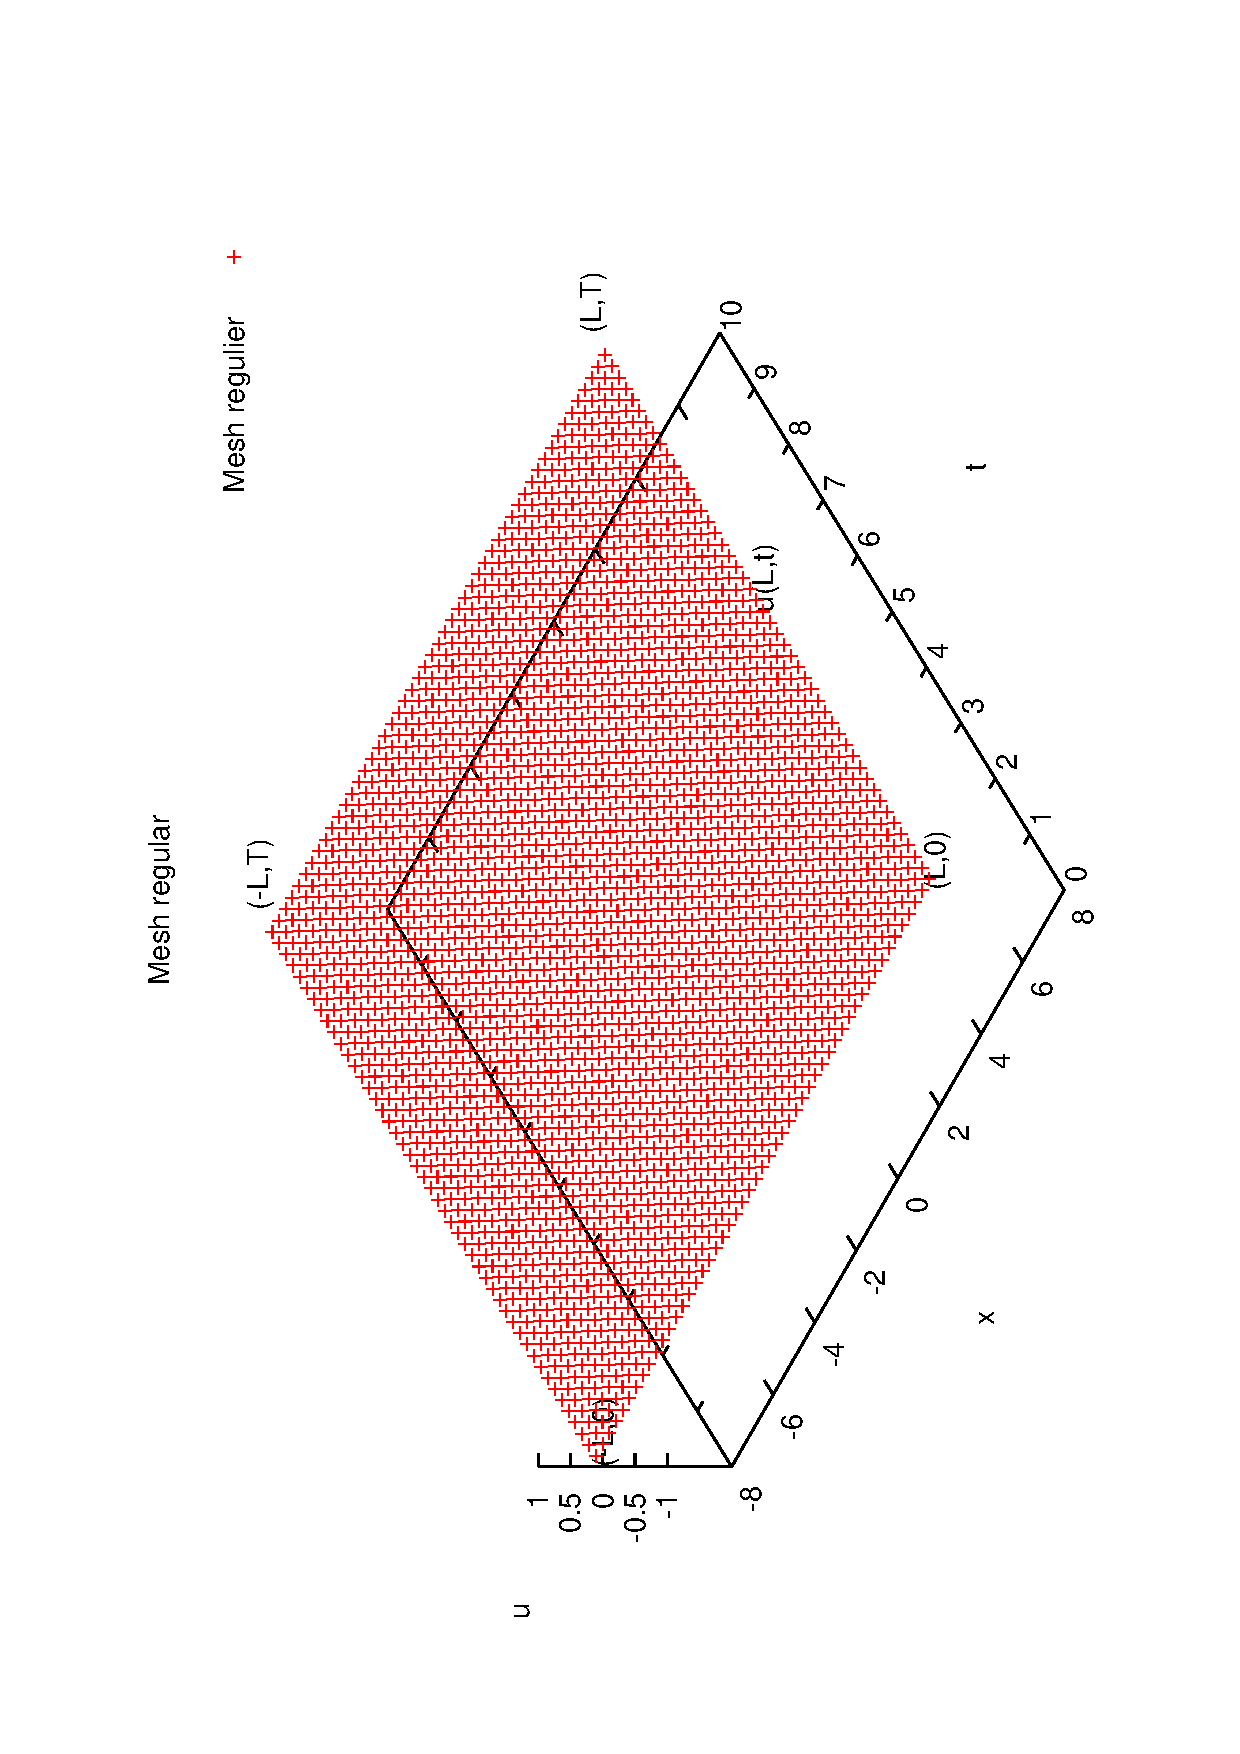
\includegraphics[ width=7cm, height=7cm,angle=-90]{MeshReg}%
 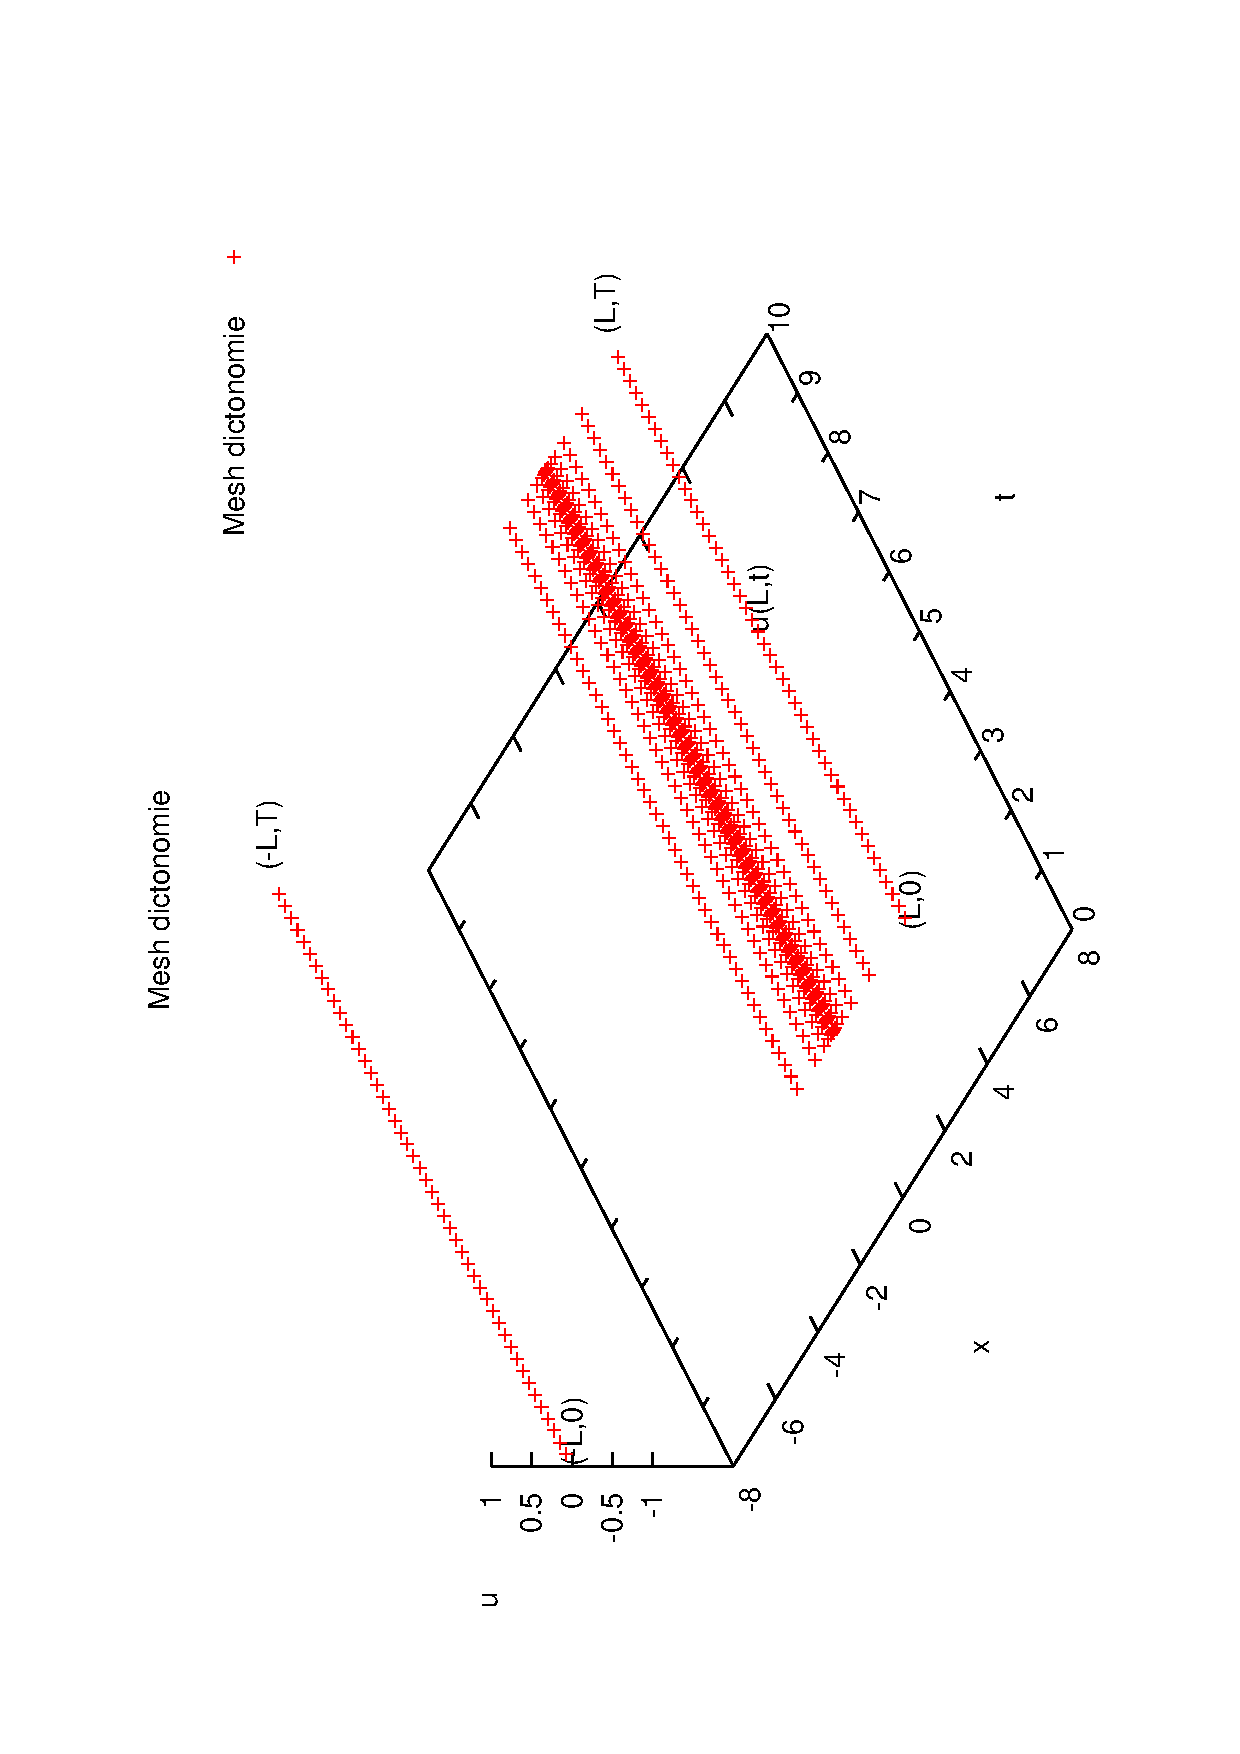
\includegraphics[ width=7cm, height=7cm,angle=-90]{MeshDicto}%
\end{center}
%%%%%%%%%%%%%%%%%%%%%%%%%%%%%%%%%%%%%%%%%%%%%%%%%%%%%%%%%%%%%%%%%%%%%%%%%%%%%%%%%%%%%%%%%
%=======================================================================================%
%%%%%%%%%%%%%%%%%%%%%%%%%%%%%%%%%%%%%%%%%%%%%%%%%%%%%%%%%%%%%%%%%%%%%%%%%%%%%%%%%%%%%%%%%
\section{Les résultats en graphique}
Par de différentes compositions de schémas et de méthodes de résolution linéaire, on a de différents résultats : \\
%==============================%
\paragraph{Schéma Euler utilisant méthode LU}
\begin{center}
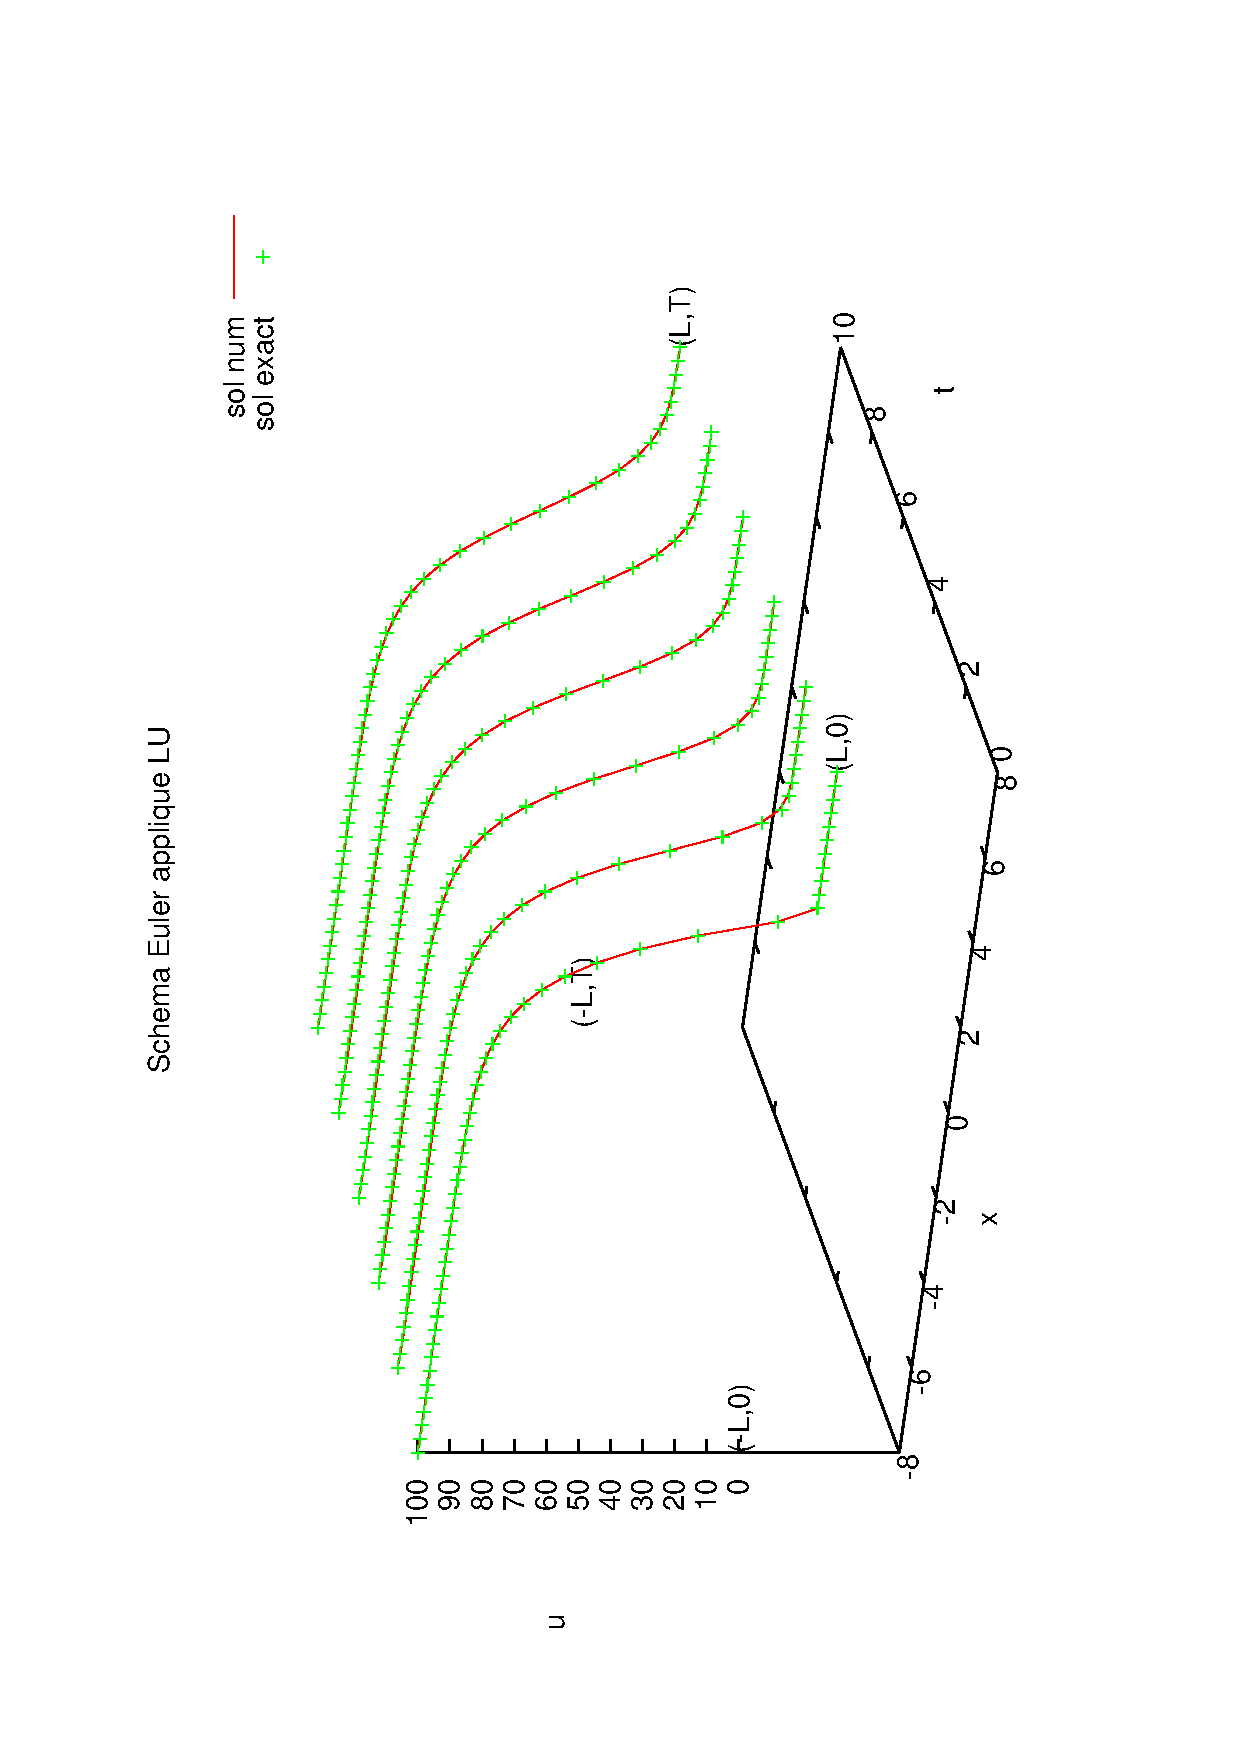
\includegraphics[angle=-90, scale=0.40]{EulerLU}%}
\end{center}
%==============================%
\paragraph{Schéma Euler utilisant méthode GC}
\begin{center}
 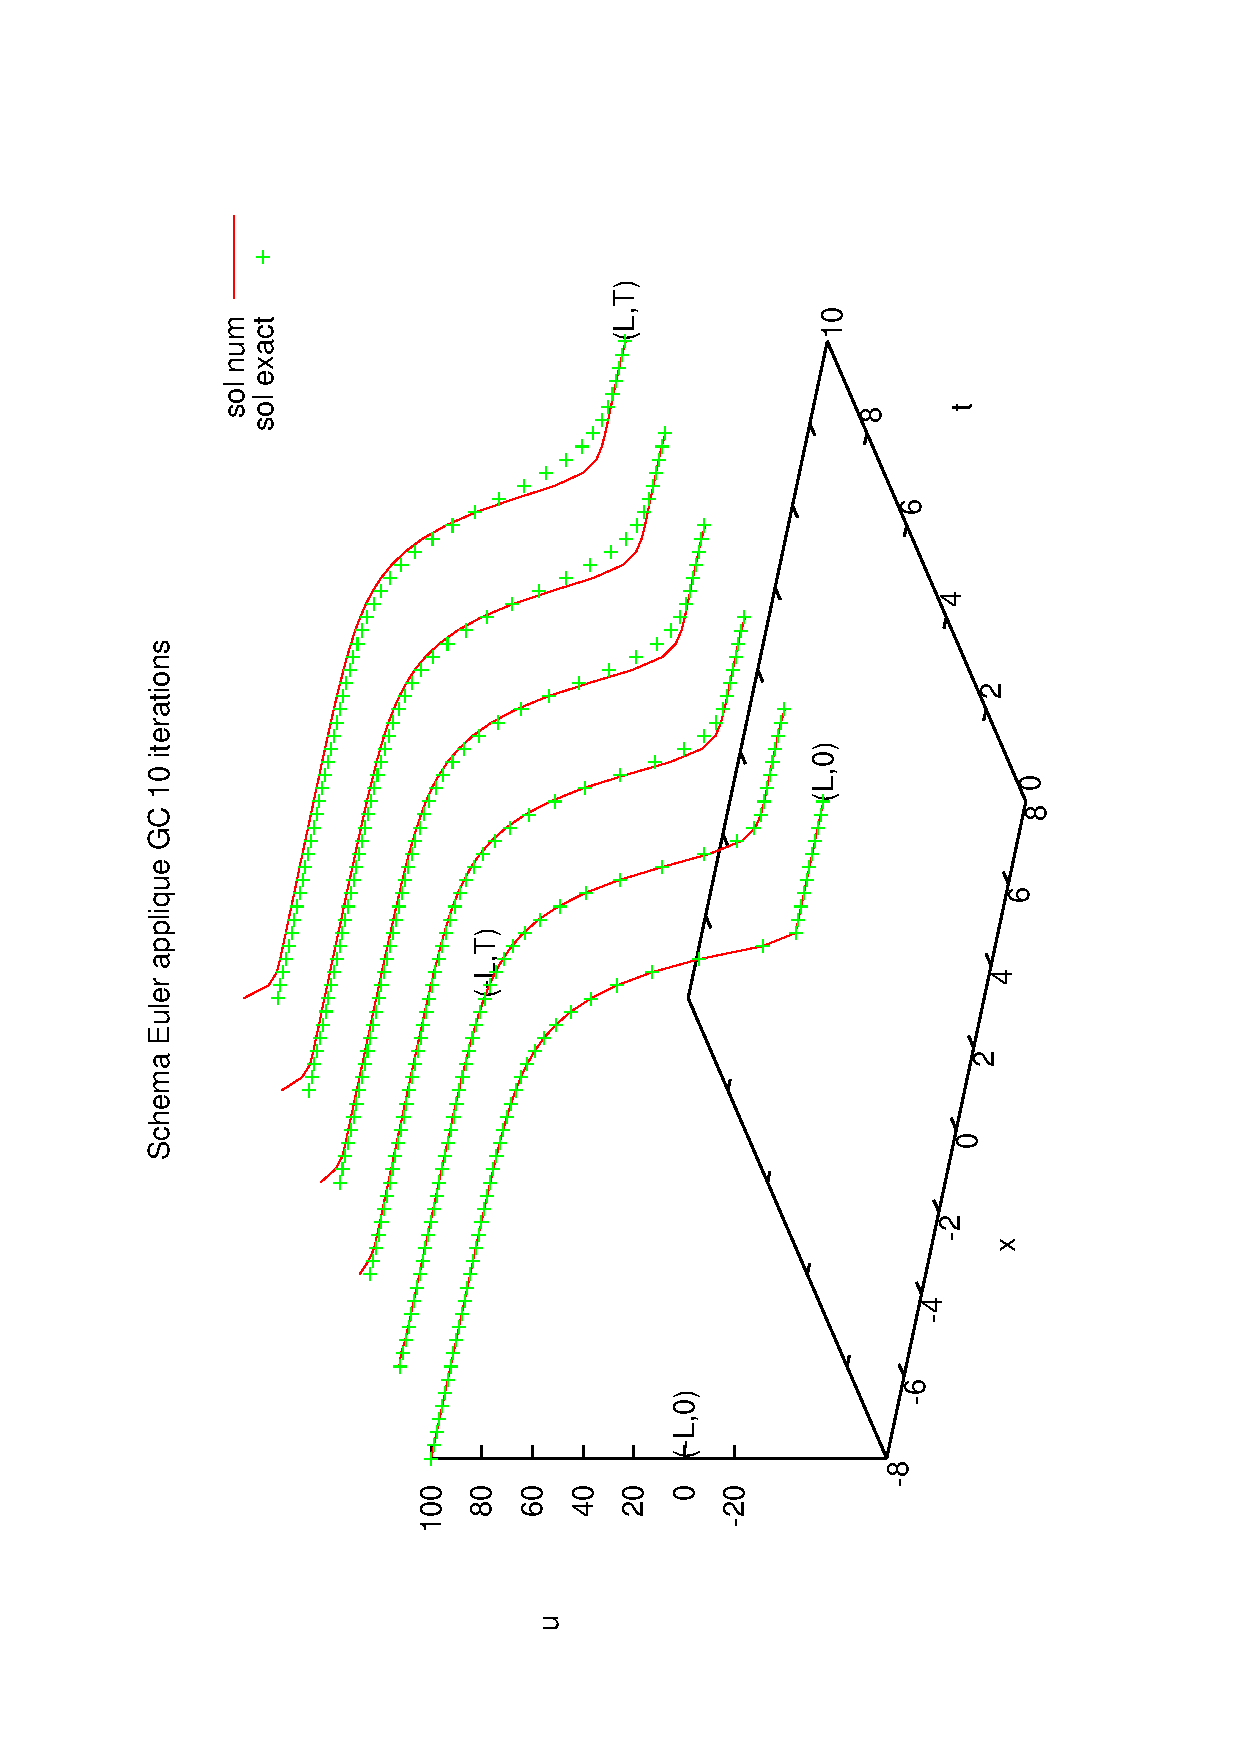
\includegraphics[ width=7cm, height=7cm,angle=-90]{EulerGC_10}%
 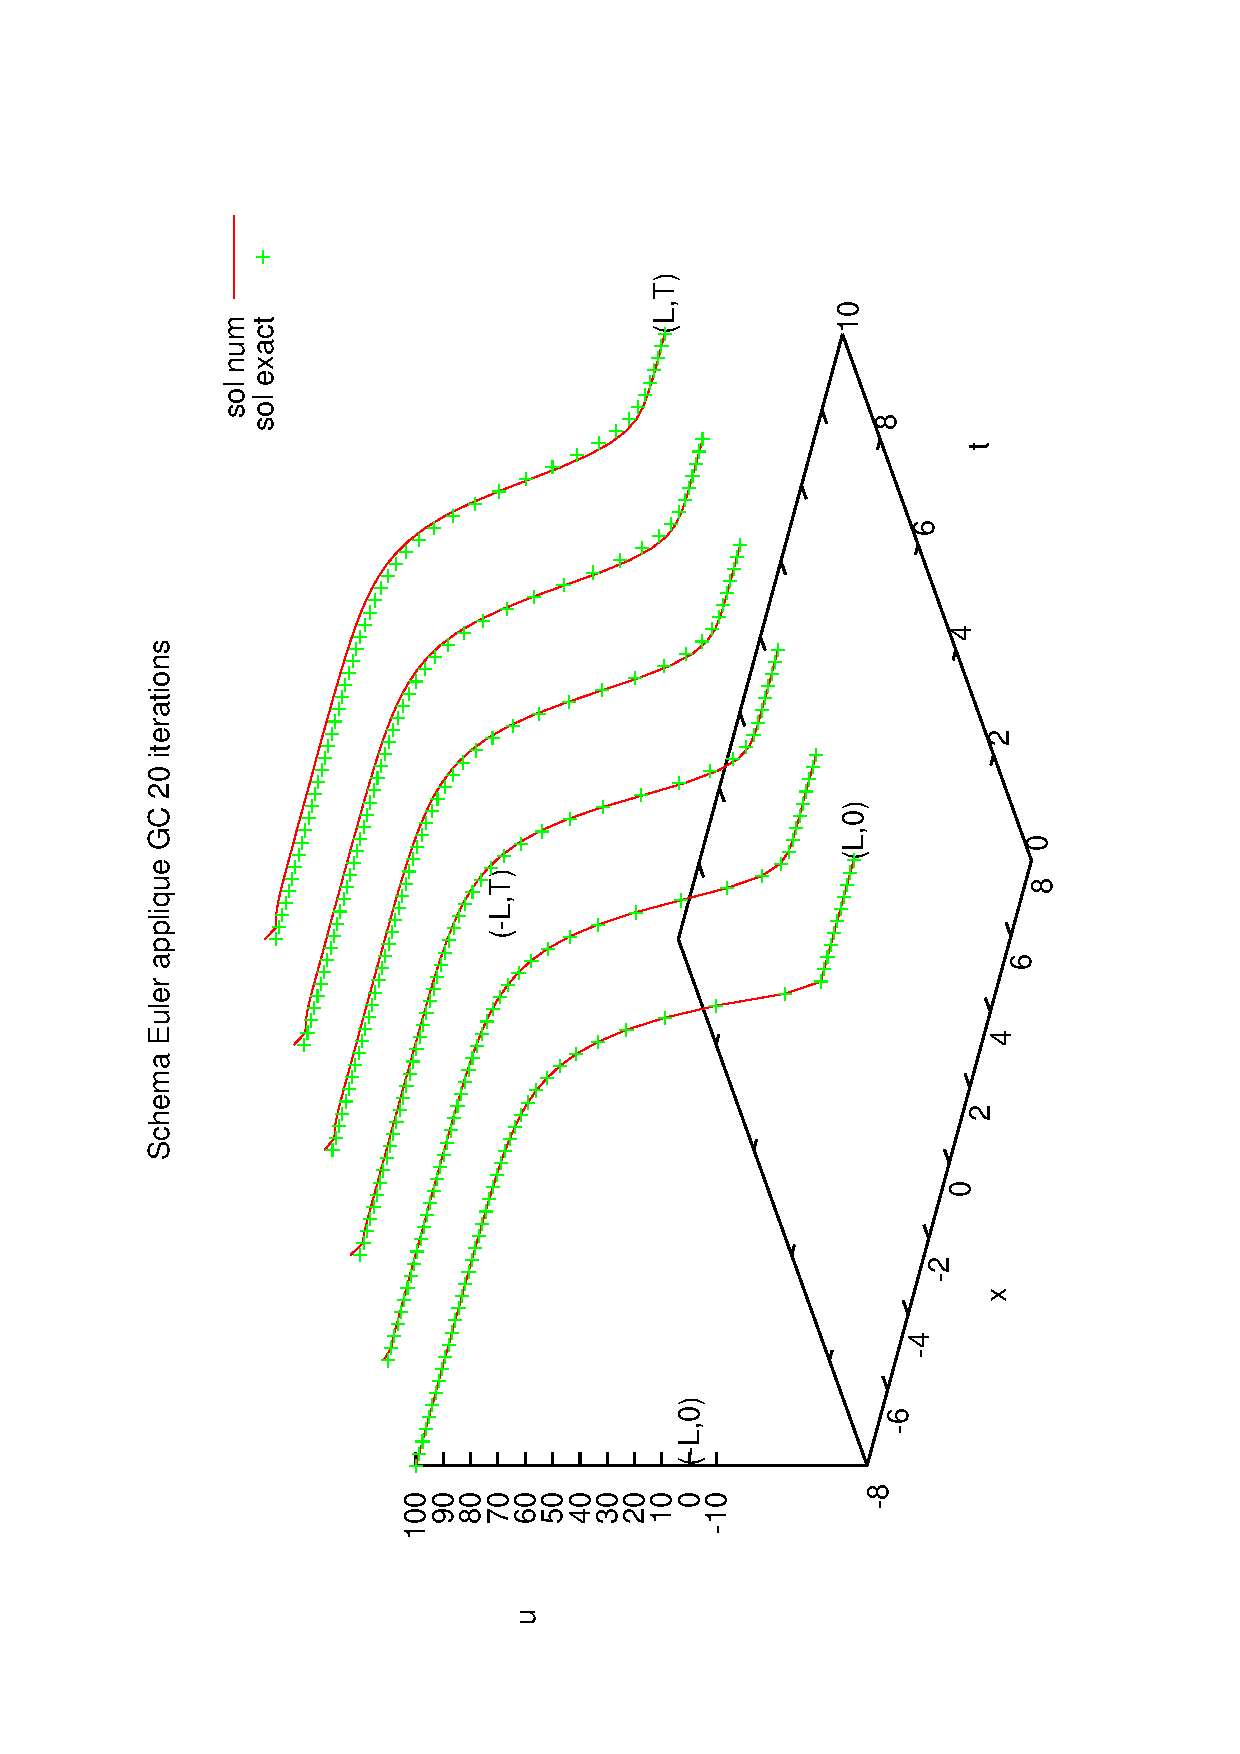
\includegraphics[ width=7cm, height=7cm,angle=-90]{EulerGC_20}%
\end{center}
%==============================%
\paragraph{Schéma Crank-Nicolson utilisant LU}
\begin{center}
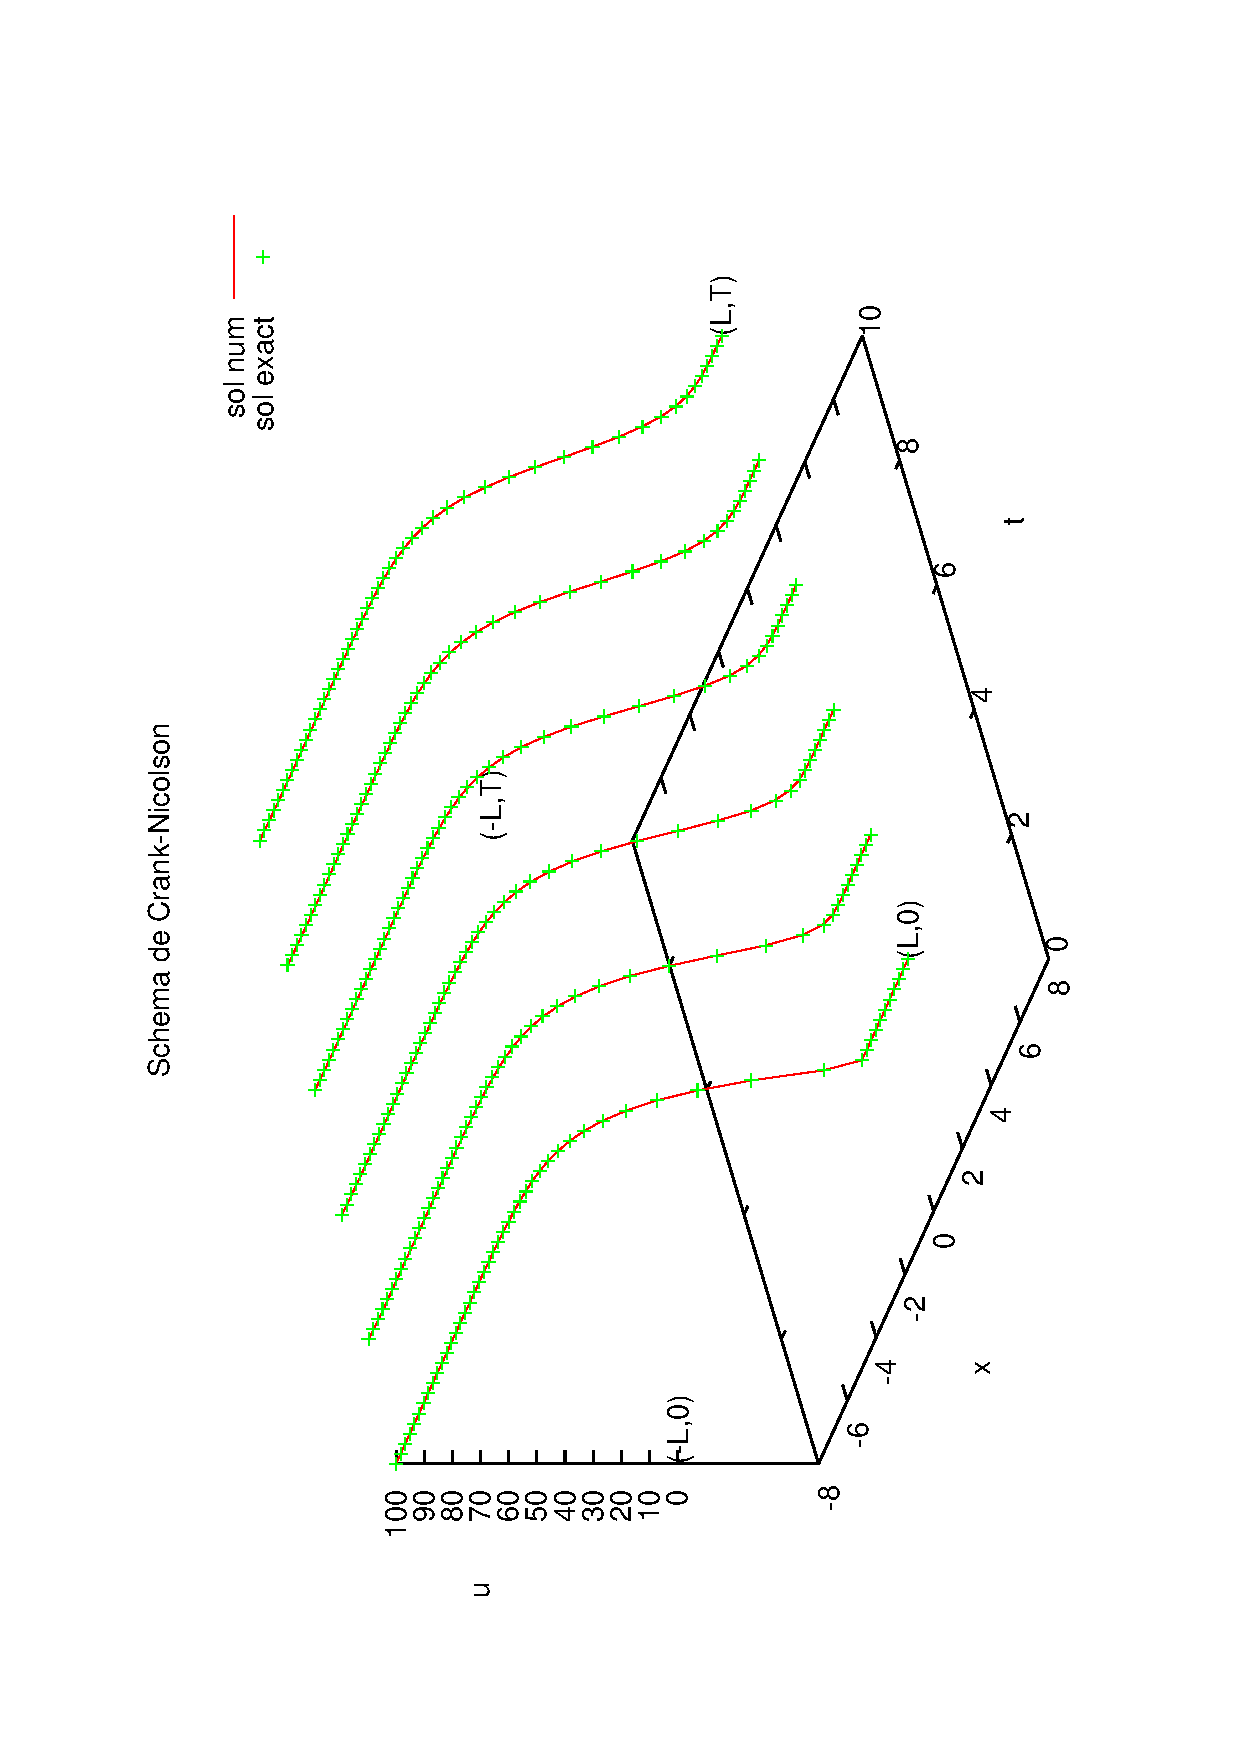
\includegraphics[angle=-90, scale=0.40]{Crank-Nicolson}%}
\end{center}
%==============================%
\paragraph{Schéma Crank-Nicolson utilisant GC}
\begin{center}
 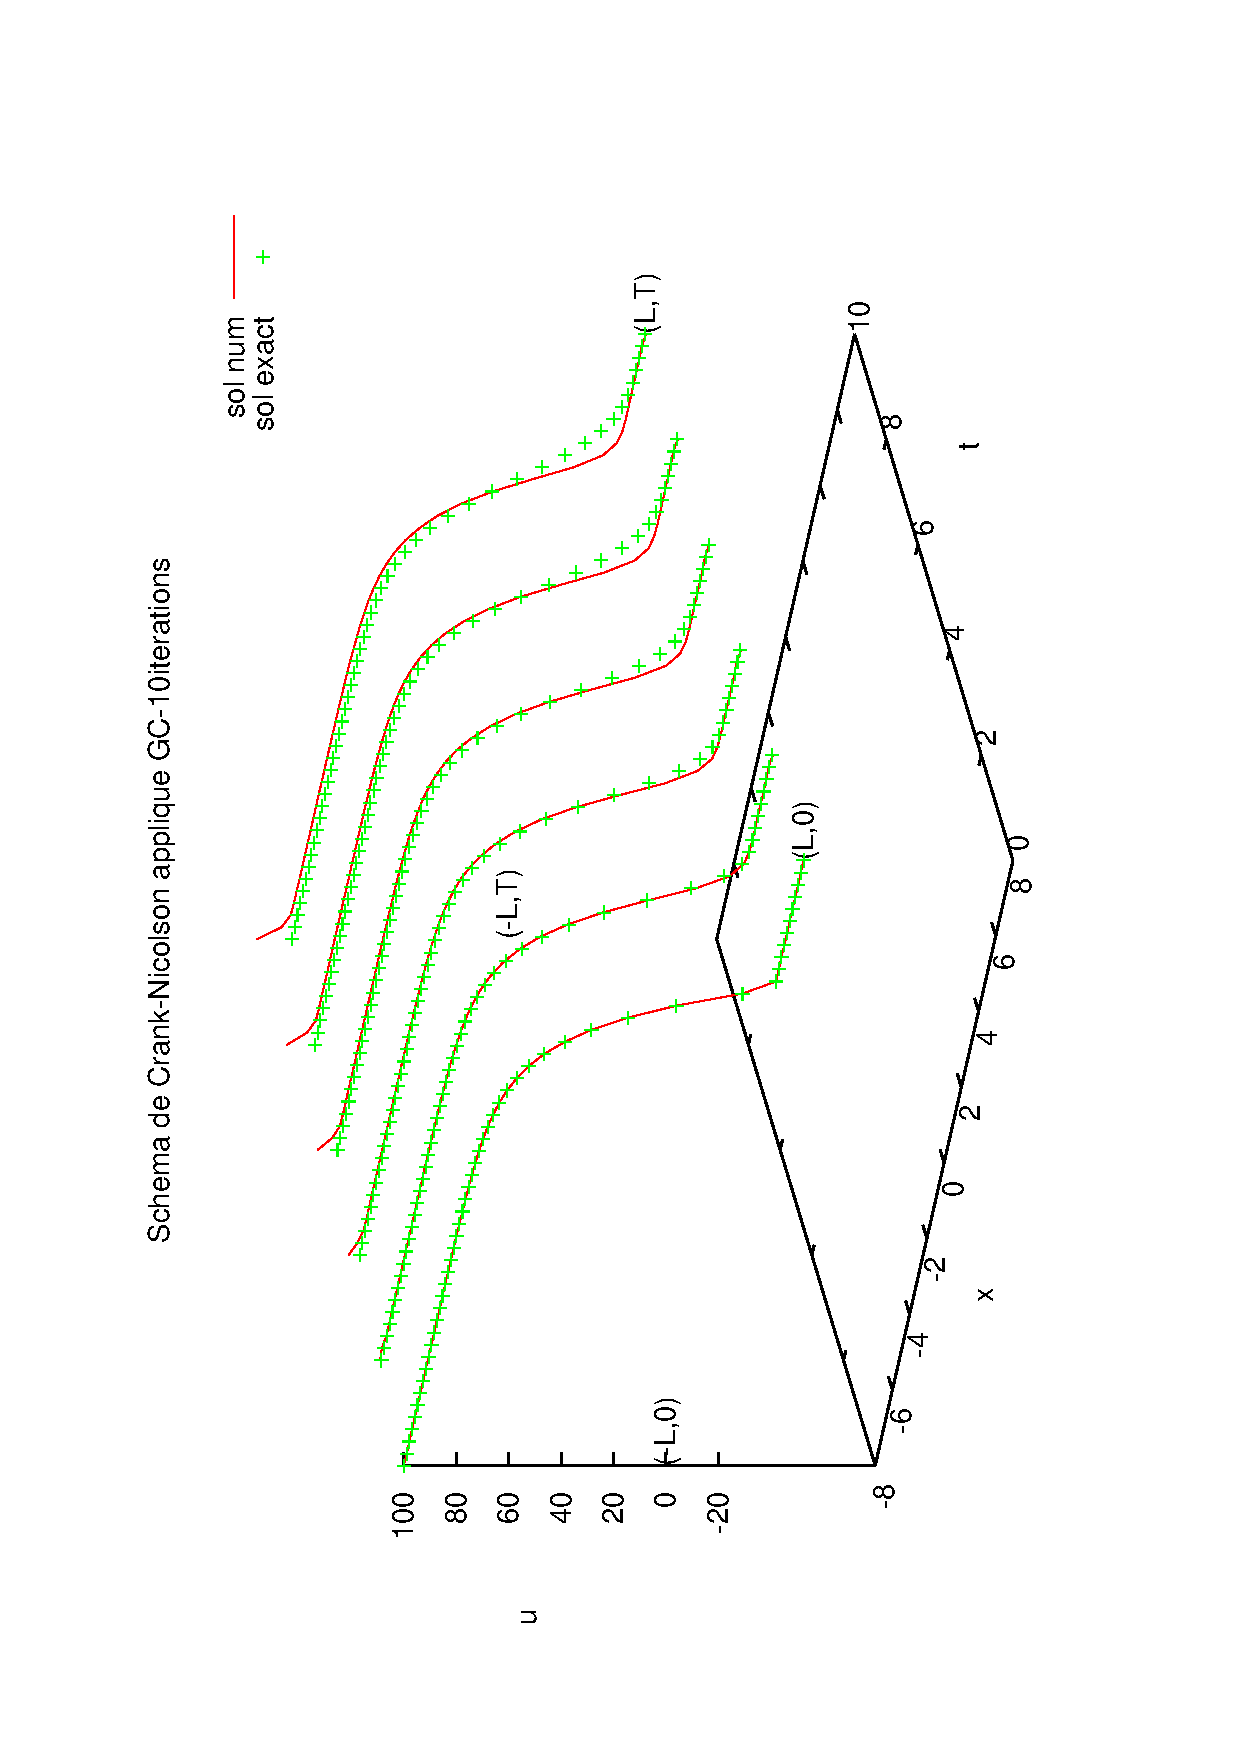
\includegraphics[ width=7cm, height=7cm,angle=-90]{Crank-Nicolson_GC10}%
 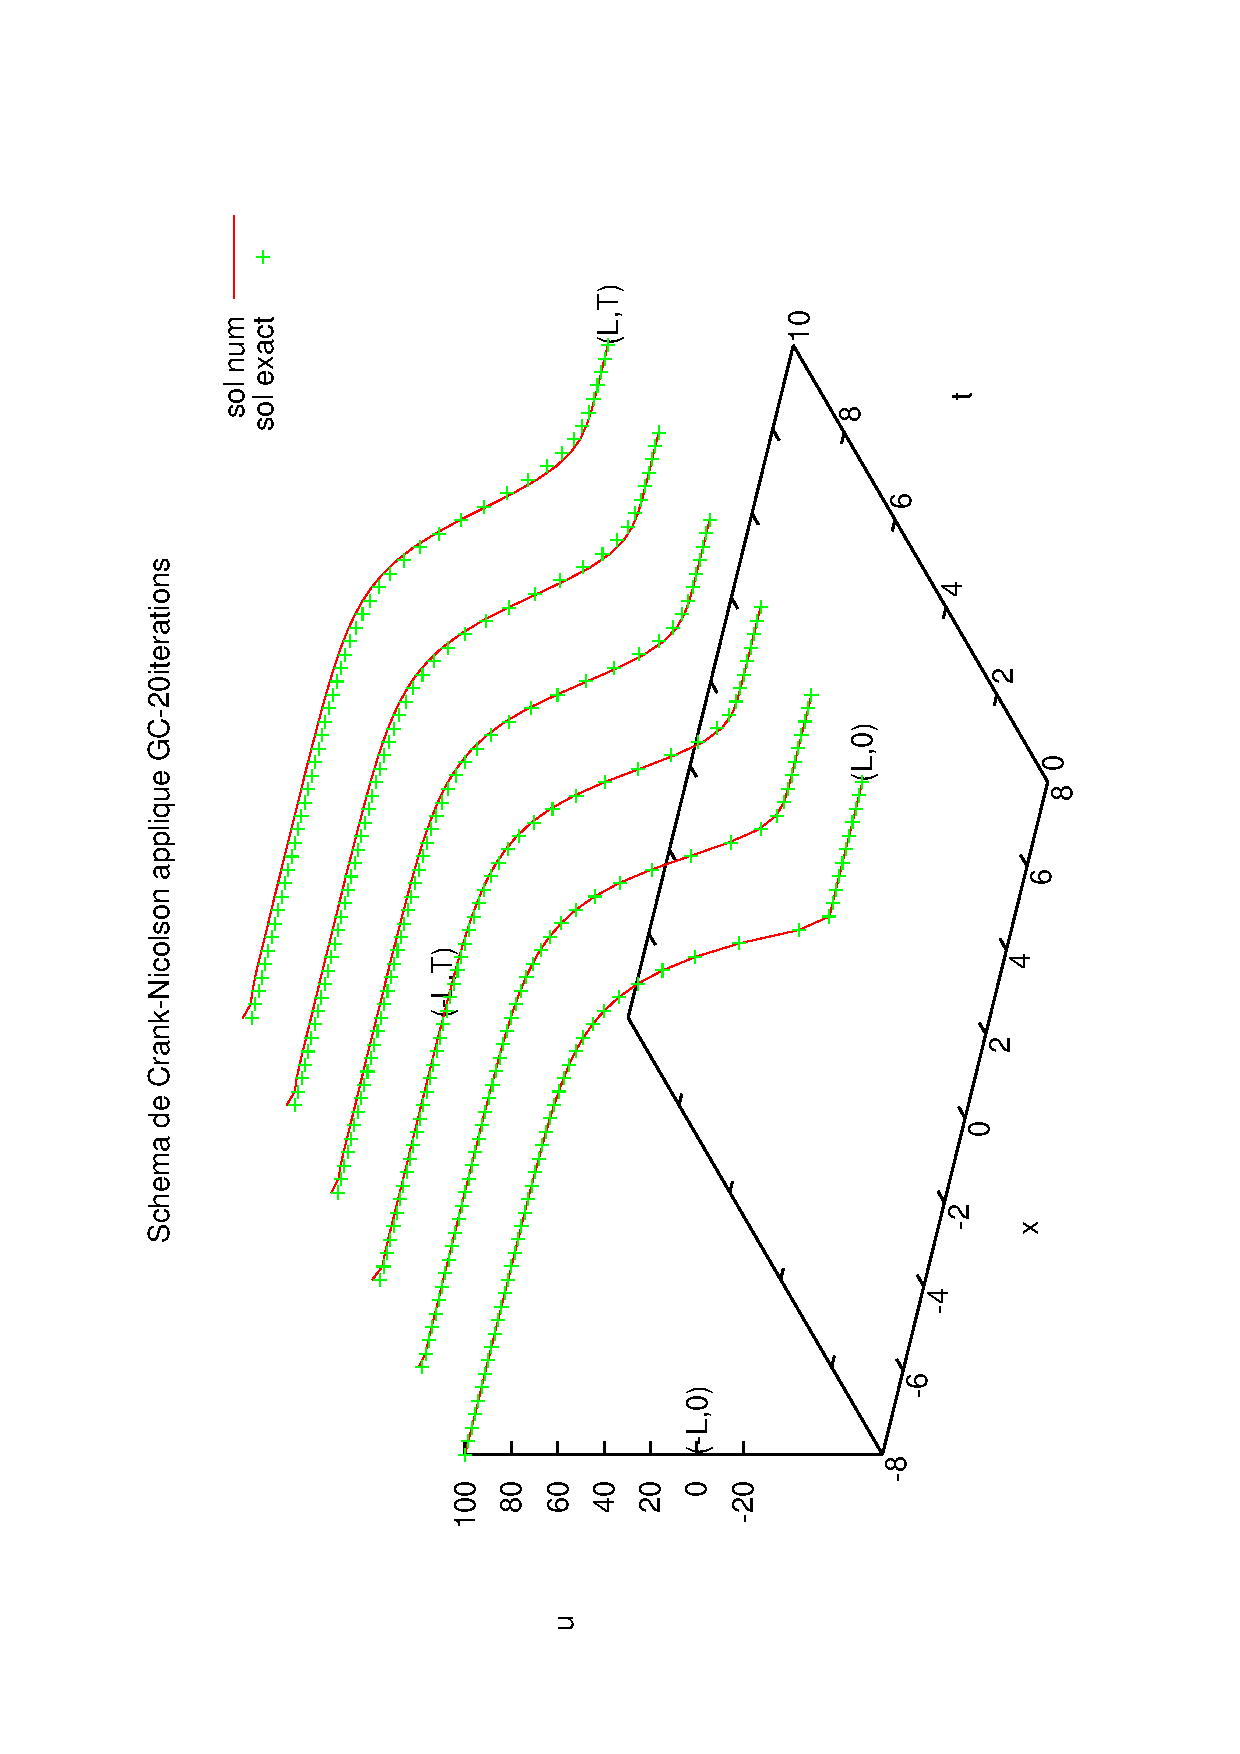
\includegraphics[ width=7cm, height=7cm,angle=-90]{Crank-Nicolson_GC20}%
\end{center}
Le Schéma de Crank-Nicolson ici est théoriquement non symétrique. Mais dans ce cas, la dissymétrie de la matrice est assez faible pour qu'il y ait lieu de la convergence de Gradient Conjugué
%==============================%
\paragraph{Gradient Conjugué divergente}
si on change $r=2$, on aura la dissymétrie forte et on ne peut plus appliquer la méthode Gradient Conjugué dans ce cas.
\begin{center}
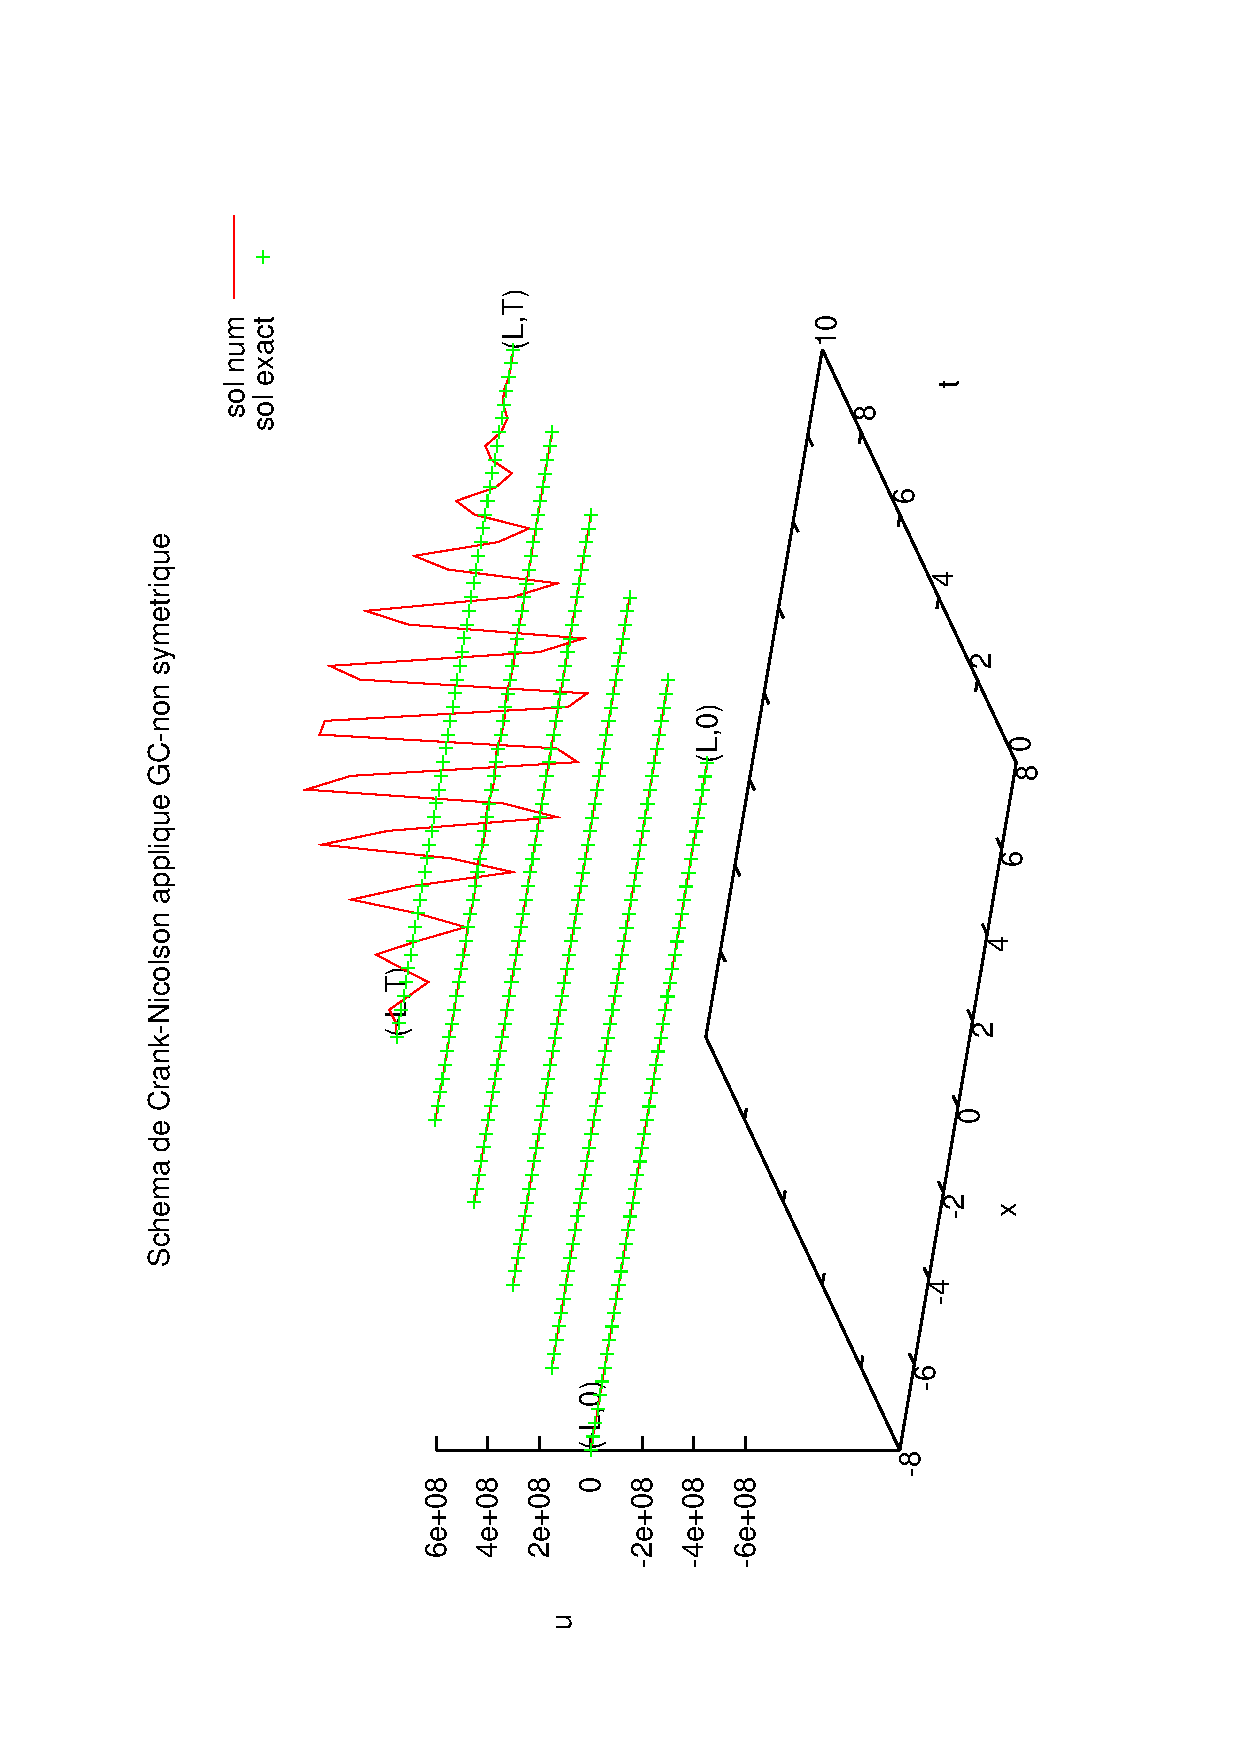
\includegraphics[angle=-90, scale=0.40]{Crank-NicolsonGCdiv}%}
\end{center}





















\chapter{Projet 2 : Pricing d'option panier sur 2 sous-jacents}
%%%%%%%%%%%%%%%%%%%%%%%%%%%%%%%%%%%%%%%%%%%%%%%%%%%%%%%%%%%%%%%%%%%%%%%%%%%%%%%%%%%%%%%%%
%=======================================================================================%
%%%%%%%%%%%%%%%%%%%%%%%%%%%%%%%%%%%%%%%%%%%%%%%%%%%%%%%%%%%%%%%%%%%%%%%%%%%%%%%%%%%%%%%%%
\section{Présentation du problème}
\paragraph{Modèle Black-Scholes : }
Le modèle Black-Schole est, à l'origine, un modèle à deux actifs : l'un risqué, l'autre pas. Typiquement, l'actif risqué est une action (l'action sous-jacente à l'option) tandis que l'actif non risqué s'apparente à une obligation. A l'instant $t$, le prix de l'obligation est $R_t$ et le prix de l'action est $S_t$. L'évolution de l'obligation est relativement simple puisque l'on suppose que :
\[
dR_t = r_tR_tdt \hspace{1cm} \hbox{soit} \hspace{1cm} R_t=R_0e^{\int_0^tr_sds}
\]
où $r_t\geq0$ représente le taux d'intérêt instantanné. Nous supposerons toujours que $R_0=1$.

Le prix de l'action, ${S_t}_{t\geq0}$ est régi par l'équation différentielle stochastique (EDS)
\[
dS_t=S_t(\mu_tdt +\sigma_tdt), \hspace{2cm} S_0\\>0\hbox{ donné,}
\]
où $\mu_t$ est un paramètre réel, et $\sigma_t\geq0$, le paramètre $\sigma$ s'appelle la volatilité.

%%%%%%%%%%%%%%%%%%%%%%%%%%%%% OK %%%%%%%%%%%%%%%%%%%%%%%%%%%%%%%%%%%%%%%
\paragraph{Pricing d'option panier sur 2 sous-jacents : }
On prend le mod{\`e}le suivant
\begin{eqnarray}&&
    \d S^1_t = S^1_t(r\d t + \d W^1_t ),
~~~%    \cr&&
    \d S^2_t = S^2_t(r\d t + \d W^2_t )
\end{eqnarray}
o{\`u} $W^1_t,W^2_t$ sont des browniens tels que
\[
    {\mathcal E}(\d W^i\d W^j) = \d t \sigma_i\sigma_j\rho_{ij}
    \hbox{ avec } =\rho_{11}=\rho_{22}=1,~~\rho_{12}=\rho_{21}=q
\]
Une option put construite sur la somme $S^1+S^2$ pour un strike $K$ et une maturit{\'e} $T$ aura donc comme prix l'esp{\'e}rance du
b{\'e}n{\'e}fice escompt{\'e}, soit
\[
    P_t = e^{-r(T-t)}{\mathcal E}(K-S^1_T-S^2_T)^+
\]
\paragraph{Equation aux d{\'e}riv{\'e}es partielles : }
D{\`e}s qu'une quantit{\'e} d{\'e}terministe d{\'e}pend de la solution d'une {\'e}quation diff{\'e}rentielle stochastique, le calcul de It{\^o} s'applique. Ici, il donne (pour une loi de probabilit{\'e} adapt{\'e}e)
$P_t = u(S^1_t, S^2_t,T-t)$  o{\`u} $u$ est la solution de
\[
\frac{\partial u}{\partial t} - \frac{\sigma_1^2 S_1^2}2\frac{\partial^2 u}{\partial S_1^2}
                    - \frac{\sigma_2^2 S_2^2}2\frac{\partial^2 u}{\partial S_2^2}
                    - q\sigma_1\sigma_2 S_1 S_2\frac{\partial^2 u}{\partial S_1\partial S_2}
                 -r S_1\frac{\partial u}{\partial S_1}-r S_2\frac{\partial u}{\partial S_2} +r u =0
\]
\[
u(S_{1},S_{2},0)=(K-S_{1}-S_{2})^{+}  \hspace{2cm} (S_{1},S_{2})\in \Re_{+}^{2}
\] 

On change de variable en posant $x=\log S_1, ~ y=\log S_2$.  Il est facile  de voir que l'{\'e}quation devient
\[
\frac{\partial u}{\partial t} - \frac{\sigma_1^2}2\frac{\partial^2 u}{\partial x^2}
                    - \frac{\sigma_2^2}2\frac{\partial^2 u}{\partial y^2}
                    - q\sigma_1\sigma_2\frac{\partial^2 u}{\partial x\partial y} +
                 \mu_1\frac{\partial u}{\partial x} + \mu_2 \frac{\partial u}{\partial y}+r u =0
\]
avec :
\[u(x,y,0)=(K-e^{x}-e^{y})^{+} \hspace{2cm} \hbox{pour tout} (x,y)\in R^{2}\].
\[\mu_{1}=\frac{\sigma_{1}^{2}}{2}-r \hspace{1cm} \hbox{et} \hspace{1cm} \mu_{2}=\frac{\sigma_{2}^{2}}{2}-r\]
%%%%%%%%%%%%%%%%%%%%%%%%%%%%%%%%%%%%%%%%%%%%%%%%%%%%%%%%%%%%%%%%%%%%%%%%%%%%%%%%%%%%%%%%%
%=======================================================================================%
%%%%%%%%%%%%%%%%%%%%%%%%%%%%%%%%%%%%%%%%%%%%%%%%%%%%%%%%%%%%%%%%%%%%%%%%%%%%%%%%%%%%%%%%%
\section{Modélisation mathématique}
Conditions aux limites :
 \[u(S_{1},S_{2},0)=(K-S_{1}-S_{2})^{+}  \hspace{2cm} (S_{1},S_{2})\in \Re_{+}^{2}\] 
Equation à résoudre : 
\[
\frac{\partial u}{\partial t}-\frac{\sigma_{1}^{2}S_{1}^{2}}{2}\frac{\partial^{2}u}{\partial S_{1}^{2}}-\frac{\sigma_{2}^{2}S_{2}^{2}}{2}\frac{\partial^{2}u}{\partial S_{2}^{2}}-q\sigma_{1}\sigma_{2}S_{1}S_{2}\frac{\partial^{2}u}{\partial S_{1}\partial S_{2}}-rS_{1}\frac{\partial u}{\partial S_{1}}-rS_{2}\frac{\partial u}{\partial S_{2}}+ru=0
\]
On effectue un changement de variables en posant $x=logS_{1},y=logS_{2}$. il est facile
de voir que l'équation devient :
\[
\frac{\partial u}{\partial t}-\frac{\sigma_{1}^{2}}{2}\frac{\partial^{2}u}{\partial x^{2}}-\frac{\sigma_{2}^{2}}{2}\frac{\partial^{2}u}{\partial y^{2}}-q\sigma_{1}\sigma_{2}\frac{\partial^{2}u}{\partial x\partial y}+\mu_{1}\frac{\partial u}{\partial x}+\mu_{2}\frac{\partial u}{\partial y}+ru=0\]
avec :
\[u(x,y,0)=(K-e^{x}-e^{y})^{+} \hspace{2cm} \hbox{pour tout} (x,y)\in R^{2}\].
\[\mu_{1}=\frac{\sigma_{1}^{2}}{2}-r \hspace{1cm} \hbox{et} \hspace{1cm} \mu_{2}=\frac{\sigma_{2}^{2}}{2}-r\]


%%%%%%%%%%%%%%%%%%%%%%%%%%%%%%%%%%%%%%%%%%%%%%%%%%%%%%%%%%%%%%%%%%%%%%%%%%%%%%%%%%%%%%%%%
%=======================================================================================%
%%%%%%%%%%%%%%%%%%%%%%%%%%%%%%%%%%%%%%%%%%%%%%%%%%%%%%%%%%%%%%%%%%%%%%%%%%%%%%%%%%%%%%%%%
\section{Résolution EDP}
%%%%%%%%%%%%%%%%%%%%%%%%%%%%%%%%%%%%%%%%%%%%%%%%%%%%%%%%%
\subsection*{Problème aux limites}
\begin{equation}
\label{limites}
\frac{\partial u}{\partial t}-\frac{\sigma_{1}^{2}}{2}\frac{\partial^{2}u}{\partial x^{2}}-\frac{\sigma_{2}^{2}}{2}\frac{\partial^{2}u}{\partial y^{2}}-q\sigma_{1}\sigma_{2}\frac{\partial^{2}u}{\partial x\partial y}+\mu_{1}\frac{\partial u}{\partial x}+\mu_{2}\frac{\partial u}{\partial y}+ru=0
\end{equation}
Conditions aux limites :
\begin{itemize}
 \item Conditions Dirichelet : 
	\[u(L,y,t)=u(x,L,t)=0 \hspace{2cm} (x,y)\in \Gamma_{N}\]
 \item Conditions Neumann    : 
	\[\kappa \nabla u.\eta =0 ~~\hbox{sur}\hspace{0.2cm}x=-L~~\hbox{et}\hspace{0.2cm}  y=-L \]
 \item Conditions initiales :
   	\[u(x,y,0)=(K-e^{x}-e^{y})^{+}  \hspace{2cm} (x,y)\in \Omega\] 
\end{itemize}

%%%%%%%%%%%%%%%%%%%%%%%%%%%%%%%%%%%%%%%%%%%%%%%%%%%%%%%%%
\subsection*{Formulation variationelle}
Soit l'espace variationel :
		\[V_{0}=\{v\in H^{1}(\Omega):v(L,y,t)=v(x,L,t)=0\}\]
Trouver $u\in V_{0}$ telle que pour tout $w\in V_{0}$, on a :
\begin{equation}
\label{variationel}
\int_{\Omega}[\frac{\partial u}{\partial t}w+\frac{\sigma_{1}^{2}}{2}\frac{\partial u}{\partial x}\frac{\partial w}{\partial x}+\frac{\sigma_{2}^{2}}{2}\frac{\partial u}{\partial y}\frac{\partial w}{\partial y}+\frac{q}{2}\sigma_{1}\sigma_{2}(\frac{\partial u}{\partial x}\frac{\partial w}{\partial y}+\frac{\partial w}{\partial x}\frac{\partial u}{\partial y})+w(\mu_{1}\frac{\partial u}{\partial x}+\mu_{2}\frac{\partial u}{\partial y}+ru)]=0
\end{equation}


%%%%%%%%%%%%%%%%%%%%%%%%%%%%%%%%%%%%%%%%%%%%%%%%%%%%%%%%%
\subsection{L'équivalence de deux problèmes}
Soit $u$ une solution suffisamment régulière du problème aux limites, $u$ appartient à $H^{2}(\Omega)$ par exemple. Alors on peut appliquer la formule de Green pour toute fonction $w$ de $H^{1}(\Omega)$, en particulier de $V_{0}$. De sorte que si on multiplie ~\eqref{limites} par $w$ de $V_{0}$, puis intégrer : 
\[
\int_{\Omega}[\frac{\partial u}{\partial t}-\hbox{div}(\kappa\nabla u)+\mu\cdot\nabla u+r u].w.d\Omega = 0
\]

\[
    \int_{\Omega}[\frac{\partial u}{\partial t} +\mu\cdot\nabla u + r u].w.d\Omega +
    \int_{\Omega}(\kappa\nabla u).\nabla w.d\Omega
    -\int_{\partial \Gamma_{N}}(\kappa\nabla u). w .\eta .d\Gamma_{N} = 0
\] 
en tenant compte que $\kappa \nabla u.\eta =0$ sur le borne de Neumann, on retrouve :
\[
    \int_{\Omega}[\frac{\partial u}{\partial t} +\mu\cdot\nabla u + r u].w.d\Omega +
    \int_{\Omega}(\kappa\nabla u).\nabla w.d\Omega = 0
\] 


Soit maintenant $u$ une solution du problème variationel. Alors pour toute fonctions $w$ de $V_{0}$, en particulier pour toute fonction de test $w$ de $D(\Omega)$, on aura :
\[
\int_{\Omega}[\frac{\partial u}{\partial t}w+\frac{\sigma_{1}^{2}}{2}\frac{\partial u}{\partial x}\frac{\partial w}{\partial x}+\frac{\sigma_{2}^{2}}{2}\frac{\partial u}{\partial y}\frac{\partial w}{\partial y}+\frac{q}{2}\sigma_{1}\sigma_{2}(\frac{\partial u}{\partial x}\frac{\partial w}{\partial y}+\frac{\partial w}{\partial x}\frac{\partial u}{\partial y})+w(\mu_{1}\frac{\partial u}{\partial x}+\mu_{2}\frac{\partial u}{\partial y}+ru)]=0
\]
On applique la formule de Green , on retrouve :
\[
\int_{\Omega}[\frac{\partial u}{\partial t}-\hbox{div}(\kappa\nabla u)+\mu\cdot\nabla u+r u].w.d\Omega = 0
\]
pour toute $w$ de $D(\Omega)$. Ce qui veut dire que $u$ satisfait ~\eqref{limites} au sens de distribution. Si on suppose en plus que $u \in H^{2}(\Omega)$ alors on peut appliquer la formule de Green pour toute fonction $w$ de $H^{1}(\Omega)$, en particulier de $V_{0}$, ce qui donne :
\[
  \int_{\Omega}[\frac{\partial u}{\partial t}-\hbox{div}(\kappa\nabla u)+\mu\cdot\nabla u+r u].w.d\Omega 
 -\int_{\partial \Gamma_{N}}(\kappa\nabla u). w .\eta .d\Gamma_{N} = 0				
\]
Par densité des traces dans l'espace $L^{2}(\partial \Omega)$, on en déduit que $u=0$ sur de borne de Neumann $L^{2}(\partial \Omega)$-p.p.

Par limite du programme, l'étude de l'existence et l'unicité de la solution du problème variationel, comme la convergence du problème variationel discret ne seront pas étudiés ici. On suppose que tout ceci a été démontrés, et on ne fait exposer que des méthodes permettant de calculer la solution dans un espace discret donné dans la suite.  
%%%%%%%%%%%%%%%%%%%%%%%%%%%%%%%%%%%%%%%%%%%%%%%%%%%%%%%%%
\subsection{Discrétisation du problème variationel}

Soit le domaine $\Omega_{h}$ possédant une triangulation $T_{h}$. L'espace discret défini par :
\[V_{h}=\{v \in C^{0}(\Omega_{h})\hspace{0.2cm},v_{|T_{k}} \in P^{1}(T_{k}),\hspace{0.2cm} v(L,y,t)=v(x,L,t)=0\}\]
Le problème variationel discret se pose : \\
Trouver $u \in V_{h}$ telle que pour toute $w \in V_{h}$, on a :
\[\int_{\Omega_{h}}[\frac{\partial u}{\partial t}w+\frac{\sigma_{1}^{2}}{2}\frac{\partial u}{\partial x}\frac{\partial w}{\partial x}+\frac{\sigma_{2}^{2}}{2}\frac{\partial u}{\partial y}\frac{\partial w}{\partial y}+\frac{q}{2}\sigma_{1}\sigma_{2}(\frac{\partial u}{\partial x}\frac{\partial w}{\partial y}+\frac{\partial w}{\partial x}\frac{\partial u}{\partial y})+w(\mu_{1}\frac{\partial u}{\partial x}+\mu_{2}\frac{\partial u}{\partial y}+ru)].d\Omega_{h}=0\]
Sachant que dans cet espace fonctionel discret, on possède des fonctions de base $w^{i}$, de sorte que pour toute $u \in V_{h}$ et toute $w \in V_{h}$, on a l'écriture : 
\[
u=\sum_{i=1}^{N_{s}} u_{i}.w^{i} \hspace{2cm} 
w=\sum_{j=1}^{N_{s}} w_{j}.w^{j} \hspace{2cm} 
N_{s} ~~\hbox{nombre de sommets}
\]
En suite, on discrétise par différence fini par rapport au temps, c'est à dire :
\[
\frac{\partial u_{i}^{m+1}}{\partial t} = \frac{u_{i}^{m+1}-u_{i}^{m}}{\partial t}
\]
Ce qui donne le schéma mixte mélanger de différences finies et éléments finis :
\[
\begin{split}
 \sum_{i=1}^{N_{s}} \int_\Omega[\frac{u_{i}^{m+1}-u_{i}^{m}}{\partial t}.w^{i}w^{j} 
 &+ u_{i}^{m+1}\frac{\sigma_1^2}2\frac{\partial w^{i}}{\partial x}\frac{\partial w^{j}}{\partial x}
 + u_{i}^{m+1}\frac{\sigma_2^2}2\frac{\partial w^{i}}{\partial y}\frac{\partial w^{j}}{\partial y}\\
 &+ u_{i}^{m+1}\frac{q}{2}\sigma_1\sigma_2(\frac{\partial w^{i}}{\partial x}\frac{\partial w^{j}}{\partial y}
 + u_{i}^{m+1}\frac{\partial w^{j}} {\partial x}\frac{\partial w^{i}}{\partial y})\\
 &+ u_{i}^{m+1}w^{j}(\mu_1\frac{\partial w^{i}}{\partial x}+\mu_2\frac{\partial w^{i}}{\partial y} +r w^{i})] =0
\end{split}
\hspace{1cm}
\forall 1 \leq j \leq N_s
\]
%%%%%%%%%%%%%%%%%%%%%%
\begin{equation}
\label{schema1}
\begin{split}
 \sum_{i=1}^{N_{s}} \int_\Omega[\frac{u_{i}^{m+1}}{\partial t}.w^{i}w^{j} 
 &+ u_{i}^{m+1}\frac{\sigma_1^2}2\frac{\partial w^{i}}{\partial x}\frac{\partial w^{j}}{\partial x}
  + u_{i}^{m+1}\frac{\sigma_2^2}2\frac{\partial w^{i}}{\partial y}\frac{\partial w^{j}}{\partial y}\\
 &+ u_{i}^{m+1}\frac{q}{2}\sigma_1\sigma_2(\frac{\partial w^{i}}{\partial x}\frac{\partial w^{j}}{\partial y}
  + u_{i}^{m+1}\frac{\partial w^{j}} {\partial x}\frac{\partial w^{i}}{\partial y})\\
 &+ u_{i}^{m+1}w^{j}(\mu_1\frac{\partial w^{i}}{\partial x}+\mu_2\frac{\partial w^{i}}{\partial y} +r w^{i})] 
  = \int_\Omega \frac{u_{i}^{m}}{\partial t}.w^{i}w^{j}
\end{split}
\hspace{1cm}
\forall 1 \leq j \leq N_s
\end{equation}
%%%%%%%%%%%%%%%%%%%%%%%
où l'écriture matricielle :
\[(M+ \delta t A) u^{m+1} = M u^m~~~\hbox{ avec } M_{ij}=\int_\Omega w^{j} w^{i}\]
Pour résoudre ce système linéaire, on se ramène dans une étude locale, i.e dans un triangle. Dans ce cas, les fonctions de base se calculent facilement par les fonctions de coordonnées barycentriques. Dans le cas de l'espace $P^1$, $w^i= \lambda_i$ avec $i=1,2,3$, les $\nabla \lambda_i$ , $\frac{\partial \lambda_i}{\partial x}$,$\frac{\partial \lambda_i}{\partial y}$ sont toutes constantes et calculables. On possède en plus une formule très générale :
\[
 \int_{T_k} (\lambda_1)^m(\lambda_2)^n(\lambda_3)^p=\frac{2|T_k|m!n!p!}{(2+m+n+p)!}
\]
Partant de ~\eqref{schema1}, on retrouve la formule matricielle :
\[  (M^k + \delta t A^k).u^{m+1} = M^k.u^m  \]
avec
\begin{equation}
\label{schema2D-matriciel}
\begin{split}
A_{ij}^k &=\int_{T_k}[\frac{1}{2}\kappa\nabla w^i.\nabla w^i +\mu.\nabla w^j w^i+ rw^i w^j].d\Omega \\
M_{ij}^k &=\int_{T_k} w^i w^j d\Omega \\
\kappa   &=\left(\begin{array}{cc}
		 \sigma_{1}^{2} & q\sigma_{1}\sigma_{2}\\
		 q\sigma_{1}\sigma_{2} & \sigma_{2}^{2}
		 \end{array}\right)
\hspace{2cm} 
\mu=\left(\begin{array}{c}
	   \mu_{1}\\
	   \mu_{2}
	  \end{array}\right)
\end{split}
\end{equation}
%%%%%%%%%%%%%%%%%%%%%%%%%%%%%%%%%%%%%%%%%%%%%%%%%%%%%%%%%
\subsection{Solution calculée}
Une fois écrit le système linéaire, on peut résoudre avec plusieurs méthodes numériques matricielles. Ici, on a deux méthodes GMRES et Gradient Conjugué. La méthode Gradient Conjugué est en général appliquable pour des matrices symétriques définies positifs. Mais dans les cas où la dissymétrie de la matrice est faible, on peut essayer de l'utiliser. La solution numérique calculée par C++ est comparée avec celle de FreeFem. L'erreur obtenu est atteint l'odre $10^{-6}$. Voici quelques images :

%\psline(0,0)(5,5)
\begin{center}
 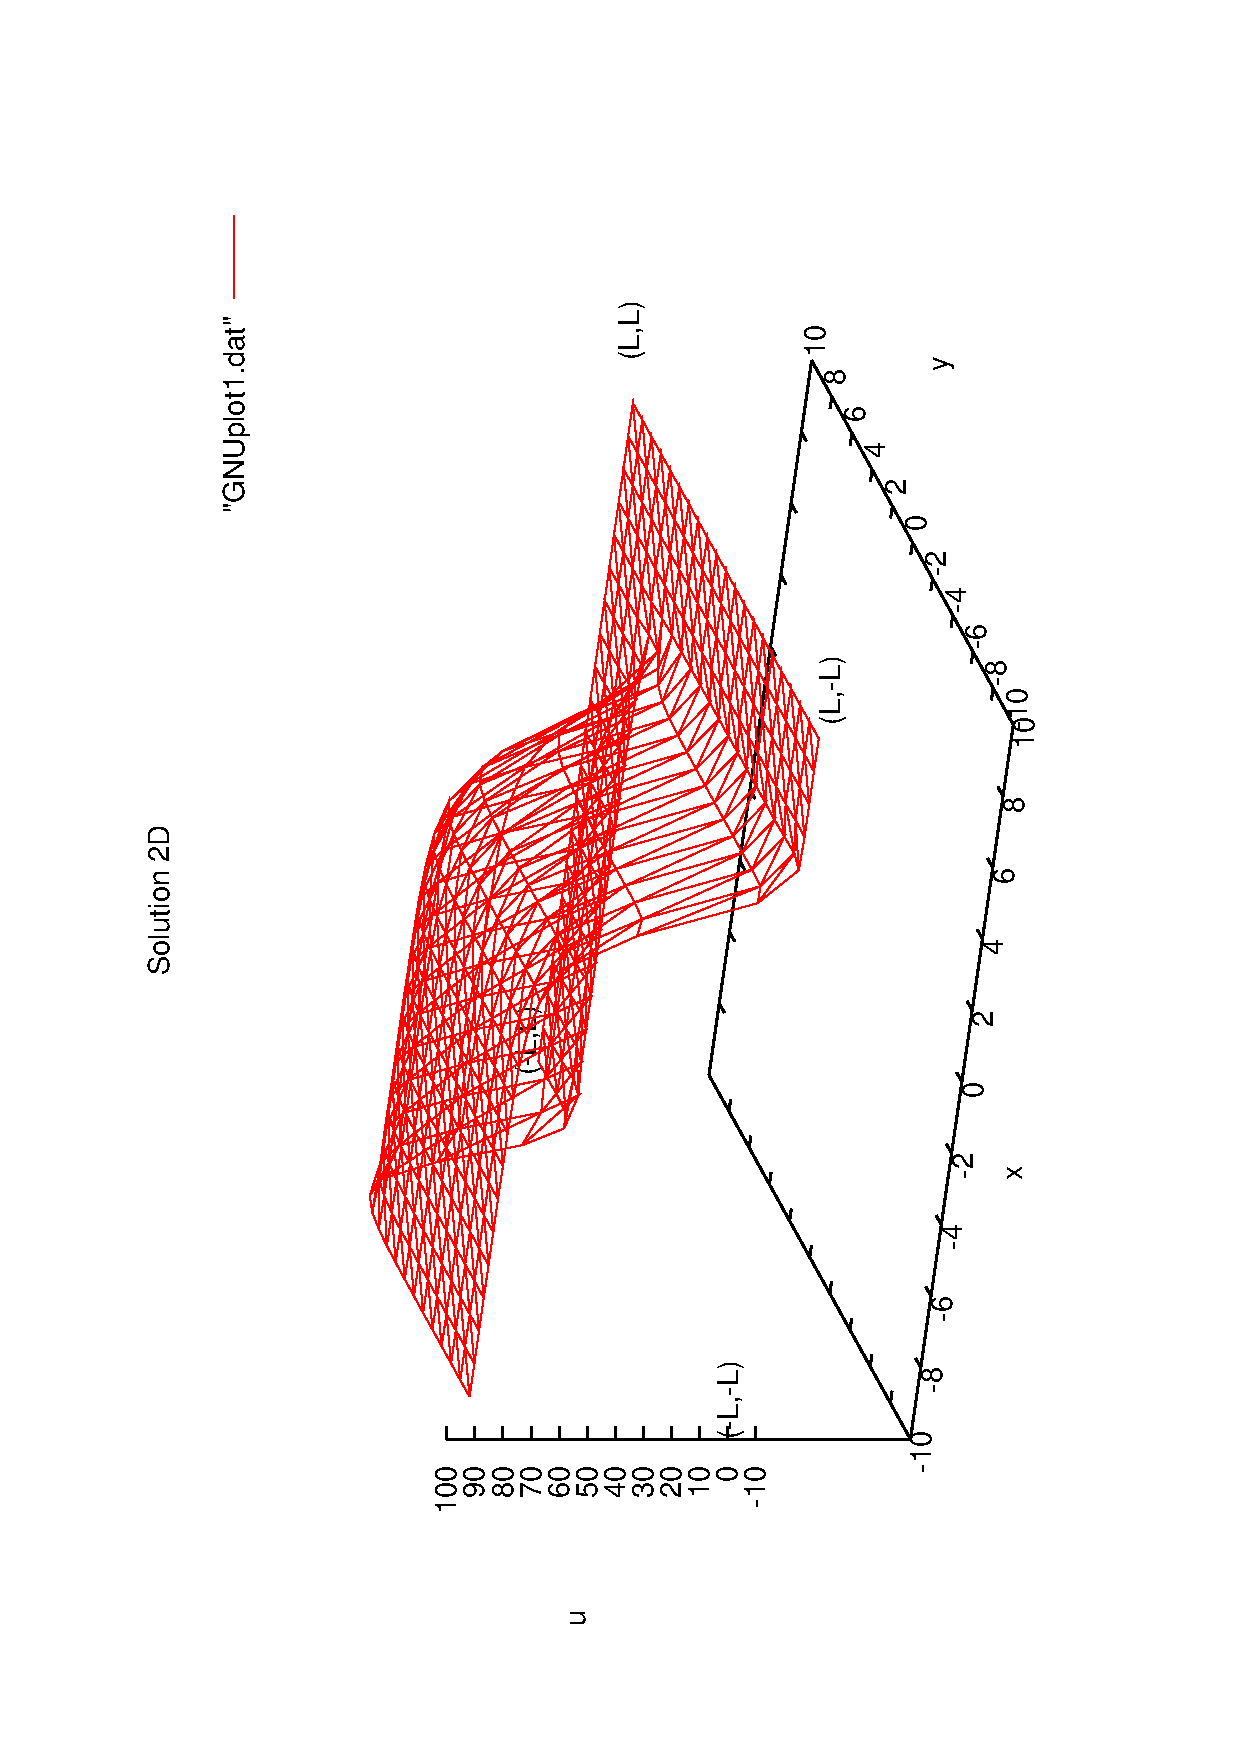
\includegraphics[ width=7cm, height=7cm]{Sol2D}%
 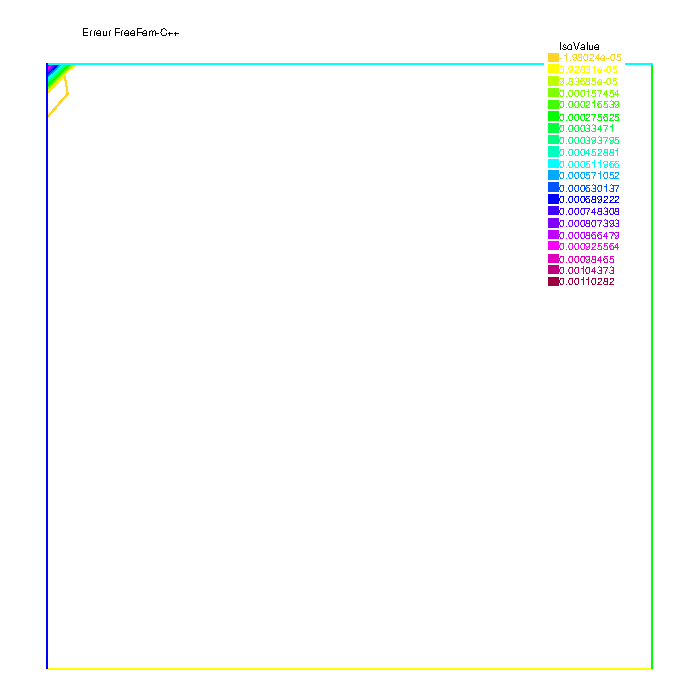
\includegraphics[ width=7cm, height=7cm]{Erreur2D}%
\end{center}
%%%%%%%%%%%%%%%%%%%%%%%%%%%%%%%%%%%%%%%%%%%%%%%%%%%%%%%%%%%%%%%%%%%%%%%%%%%%%%%%%%%%%%%%%
%=======================================================================================%
%%%%%%%%%%%%%%%%%%%%%%%%%%%%%%%%%%%%%%%%%%%%%%%%%%%%%%%%%%%%%%%%%%%%%%%%%%%%%%%%%%%%%%%%%
\section{Etude locale de la solution 2D}
Maintenant, on a trouvé la solution numérique sur le maillage donné. Une question à poser est : quelle est la valeur de $u$ sur un point donné. Le calcul s'effectue sur 2 étape :
\begin{itemize}
 \item localisation du point sur le maillage, i.e le point est dans quel triangle
 \item calcul localement la valeur de $u$ sur ce point.
\end{itemize} \par
Première étape : soit un point $P$ donné. On va parcourir tous les triangles du maillage en testant si le point $P$ est dans un triangle. Pour ce test, on a deux méthodes. La première consiste à calculer la surface (toujours positif) des trois triangles formés par le point $P$ et les trois sommets du triangle $T_k$ du maillage. Si la somme de ces trois surface est exactement 1, le point $P$ est alors dans le triangle $T_k$. La deuxième méthode consiste à utiliser les fonctions de coordonnées barycentriques. Un point $P$ et un triangle $T_k$ donnés forme trois coordonnées barycentriques $\lambda_i$, $i=1,2,3$. Si ces trois coordonnées sont toutes positives, le point $P$ est dans le triangle $T_k$.\par
Deuxième étape : Le triangle $T_k$ qui contient le point $P$ a été trouvé. On possède les trois fonctions de coordonnées barycentriques $\lambda_i$, $i=1,2,3$, avec les valeurs  $u_i$ , $i=1,2,3$ sur les sommets de ce triangle. Alors                 \[u(P)=\sum_{i=1}^3\lambda_i . u_i\]
\begin{center}
 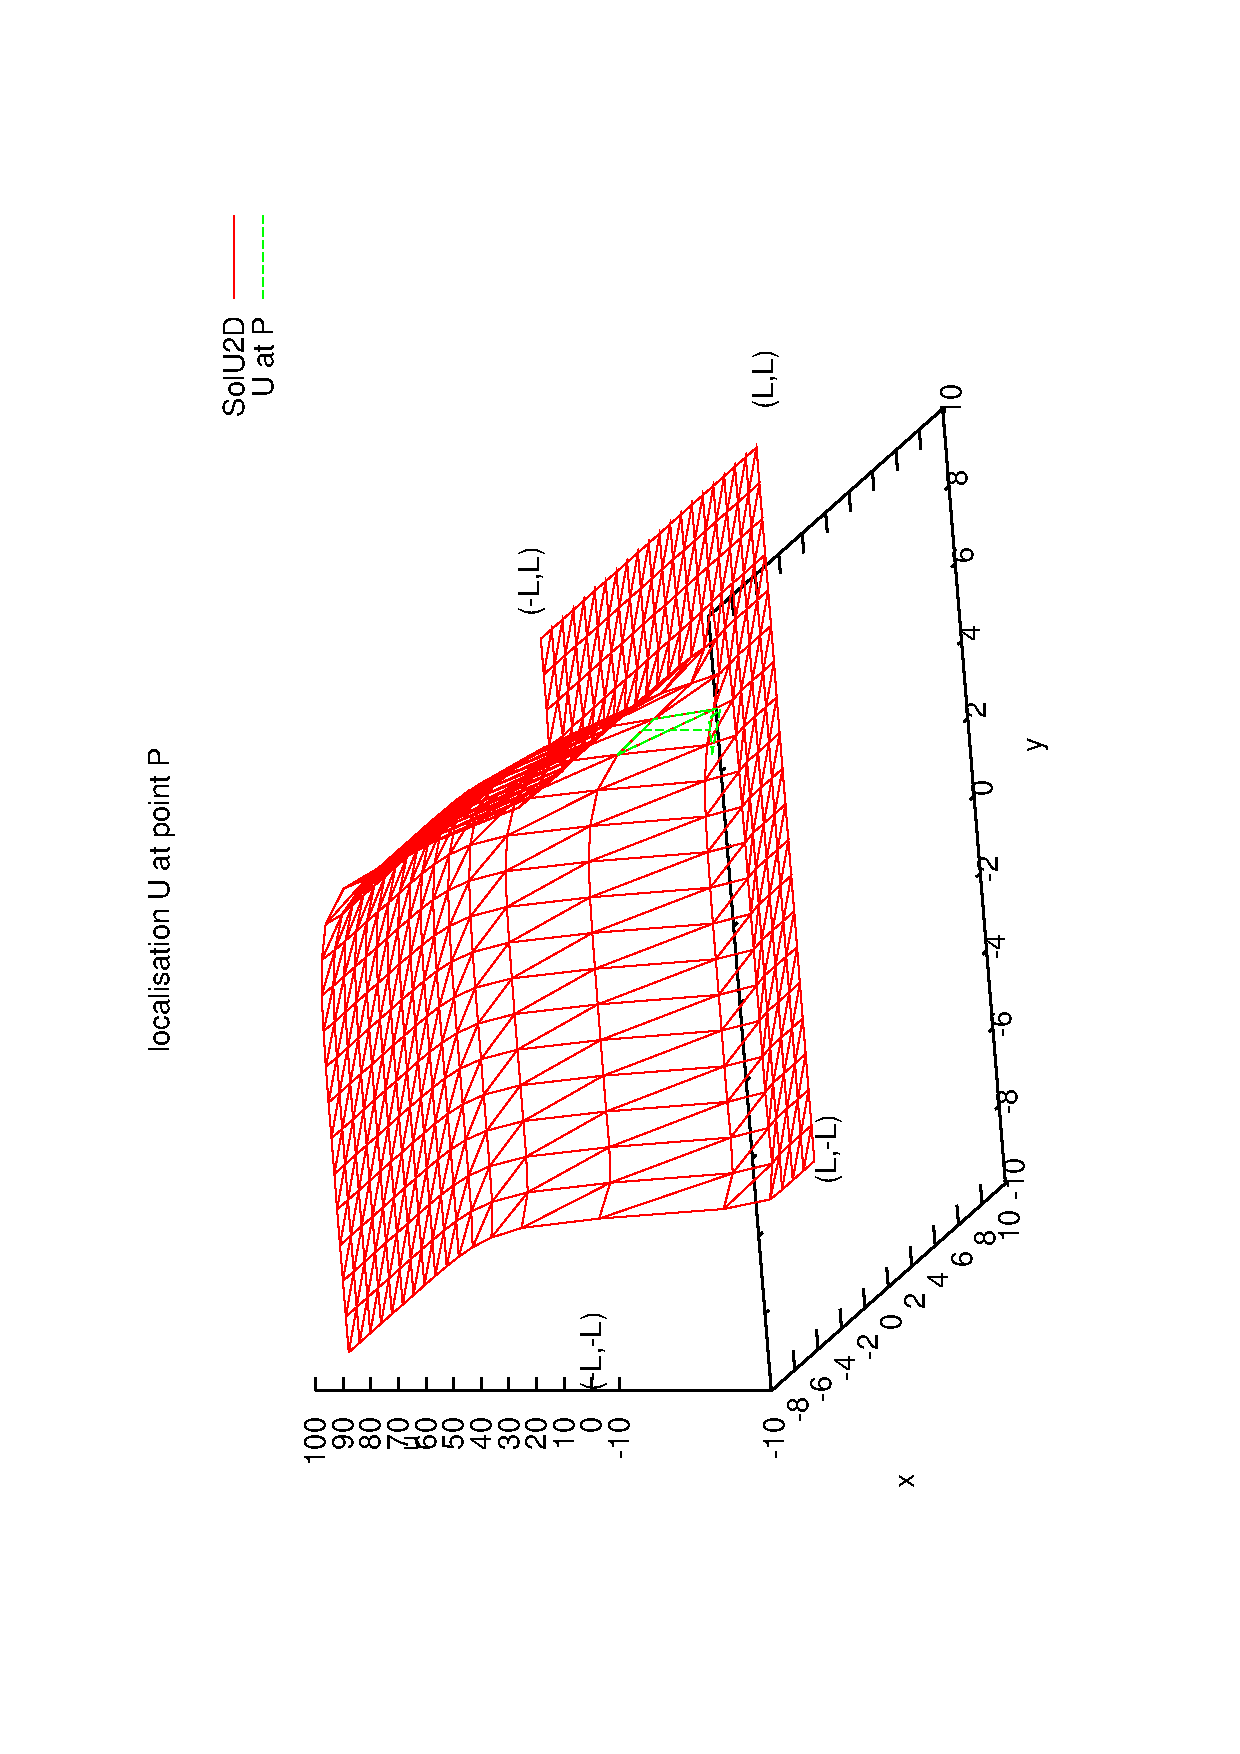
\includegraphics[ width=7cm, height=7cm, angle=-90]{UatP}%
\end{center}
%%%%%%%%%%%%%%%%%%%%%%%%%%%%%%%%%%%%%%%%%%%%%%%%%%%%%%%%%%%%%%%%%%%%%%%%%%%%%%%%%%%%%%%%%
%=======================================================================================%
%%%%%%%%%%%%%%%%%%%%%%%%%%%%%%%%%%%%%%%%%%%%%%%%%%%%%%%%%%%%%%%%%%%%%%%%%%%%%%%%%%%%%%%%%
\section{Etude différentielle de la solution 2D}
%%%%%%%%%%%%%%%%%%%%%%%%%%%%%%%%%%%%%%%%%%%%%%%%%%%%%%%%%%%%%%%%%%%%%%%%%%%%%%%%%%%%%%%%%%
\subsection{Différence fini}
Par la formule de Taylor :
               \[\begin{split}
			u(x+\Delta x)&=u(x)+ \Delta x.u'(x) +o(\Delta x) \\
		        u(x-\Delta x)&=u(x)- \Delta x.u'(x) +o(\Delta x) 
		\end{split}\]
On peut approximer la dérivée par rapport à $K$ et à $q$ par :
\[
	\begin{split}
		\frac{\partial u}{\partial K} &\approx \frac{u(K)-u(K-\Delta K)}{\Delta K}\\
		\frac{\partial u}{\partial q} &\approx \frac{u(q)-u(q-\Delta q)}{\Delta q}
	\end{split}
\]
Ou bien par différence centrée :
\[
	\begin{split}
		\frac{\partial u}{\partial K} &\approx \frac{u(K+\Delta K)-u(K-\Delta K)}{2\Delta K}\\
		\frac{\partial u}{\partial q} &\approx \frac{u(q+\Delta q)-u(q-\Delta q)}{2\Delta q}
	\end{split}
\]
%%%%%%%%%%%%%%%%%%%%%%%%%%%%%%%%%%%%%%%%%%%%%%%%%%%%%%%%%%%%%%%%%%%%%%%%%%%%%%%%%%%%%%%%%%
\subsection{Différentiation automatique}
Comme son nom indique, la Différentiation automatique est une méthode permettant de calculer certaines dérivées numériques d'une fonction automatiquement. Il existe plusieurs bibliothèques pour plusieurs languages pour effectuer ces calculs. On possède ici les bibliothèques ddouble.hpp et R2ddouble.hpp, qui permet de calculer dans les cas réels et $R^2$ dans le language C++. L'importance est la bonne déclaration des variables concernant les calculs. 
\subsection*{graphique}
\begin{center}
 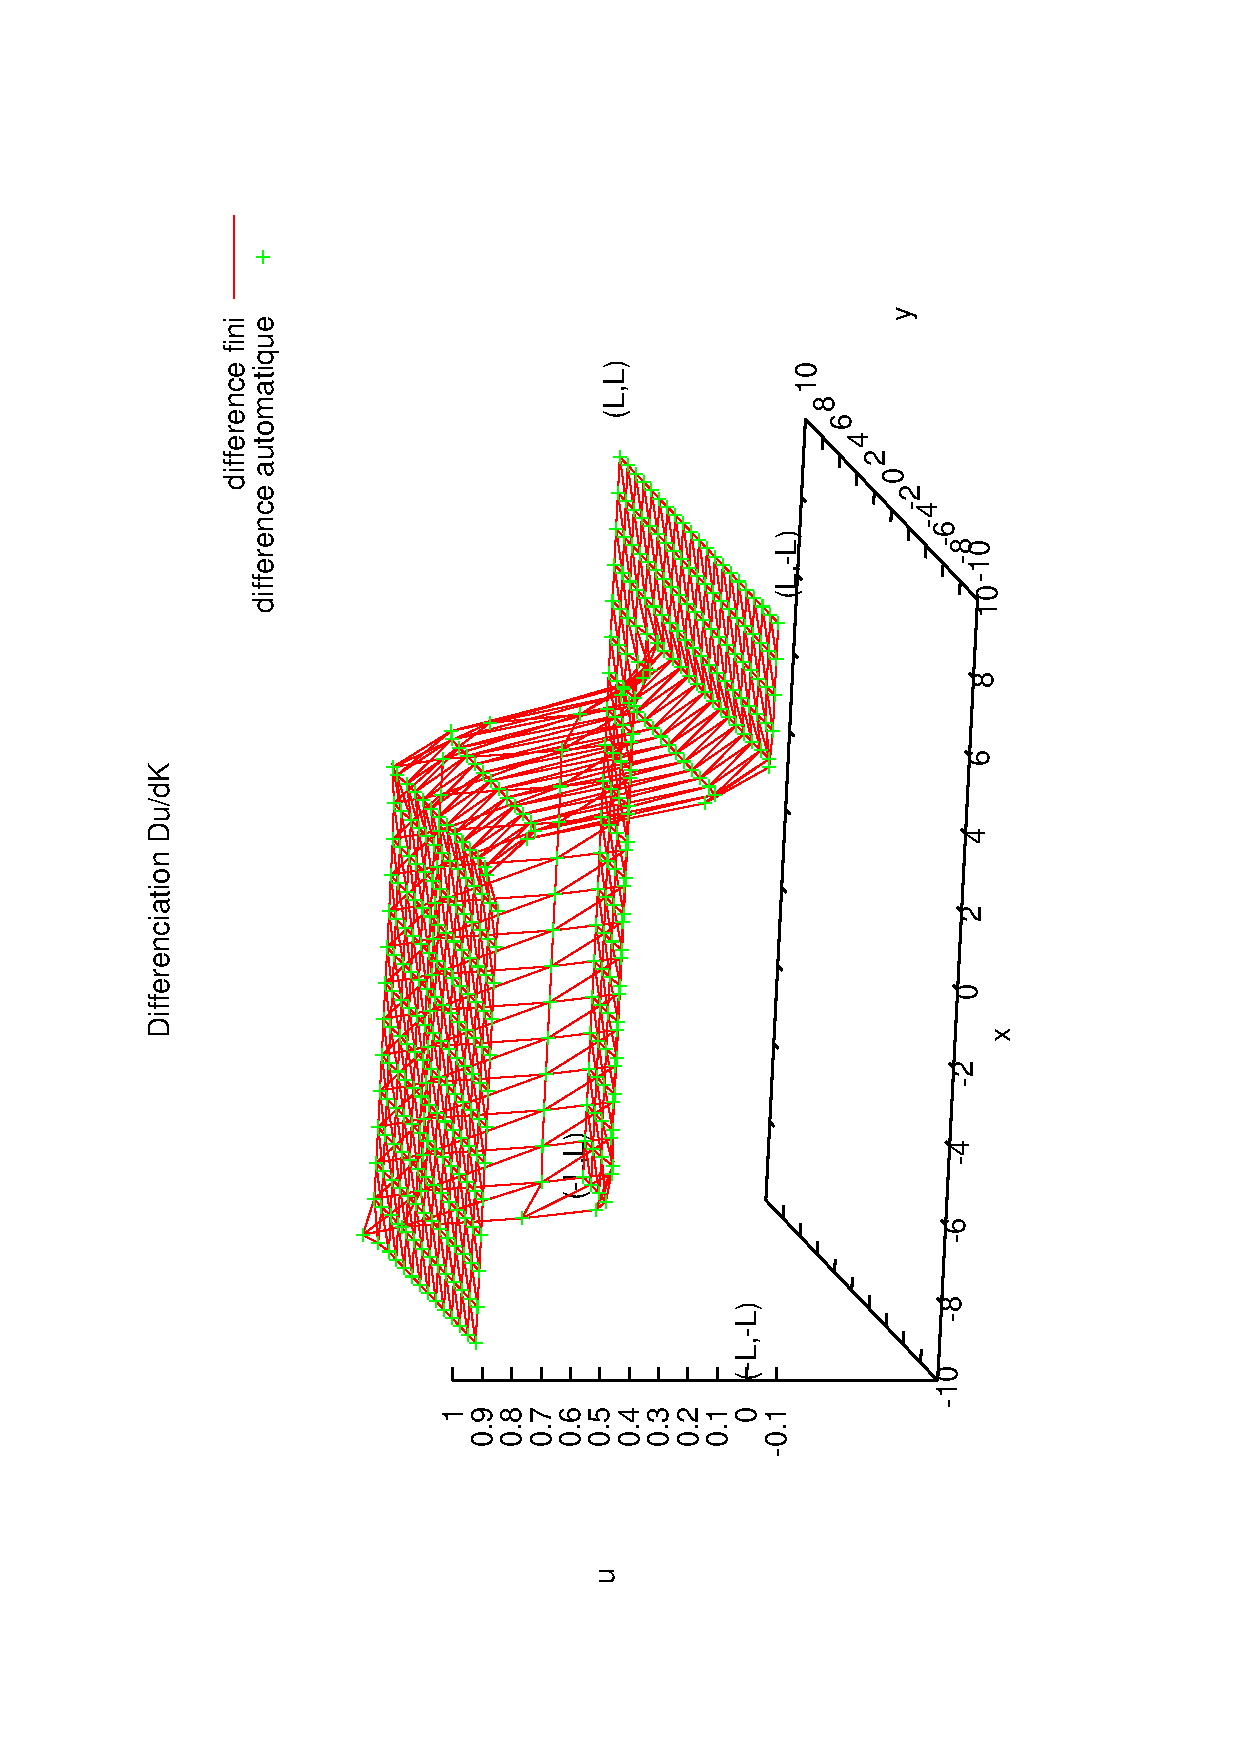
\includegraphics[ width=7cm, height=7cm,angle=-90]{DUdK}%
 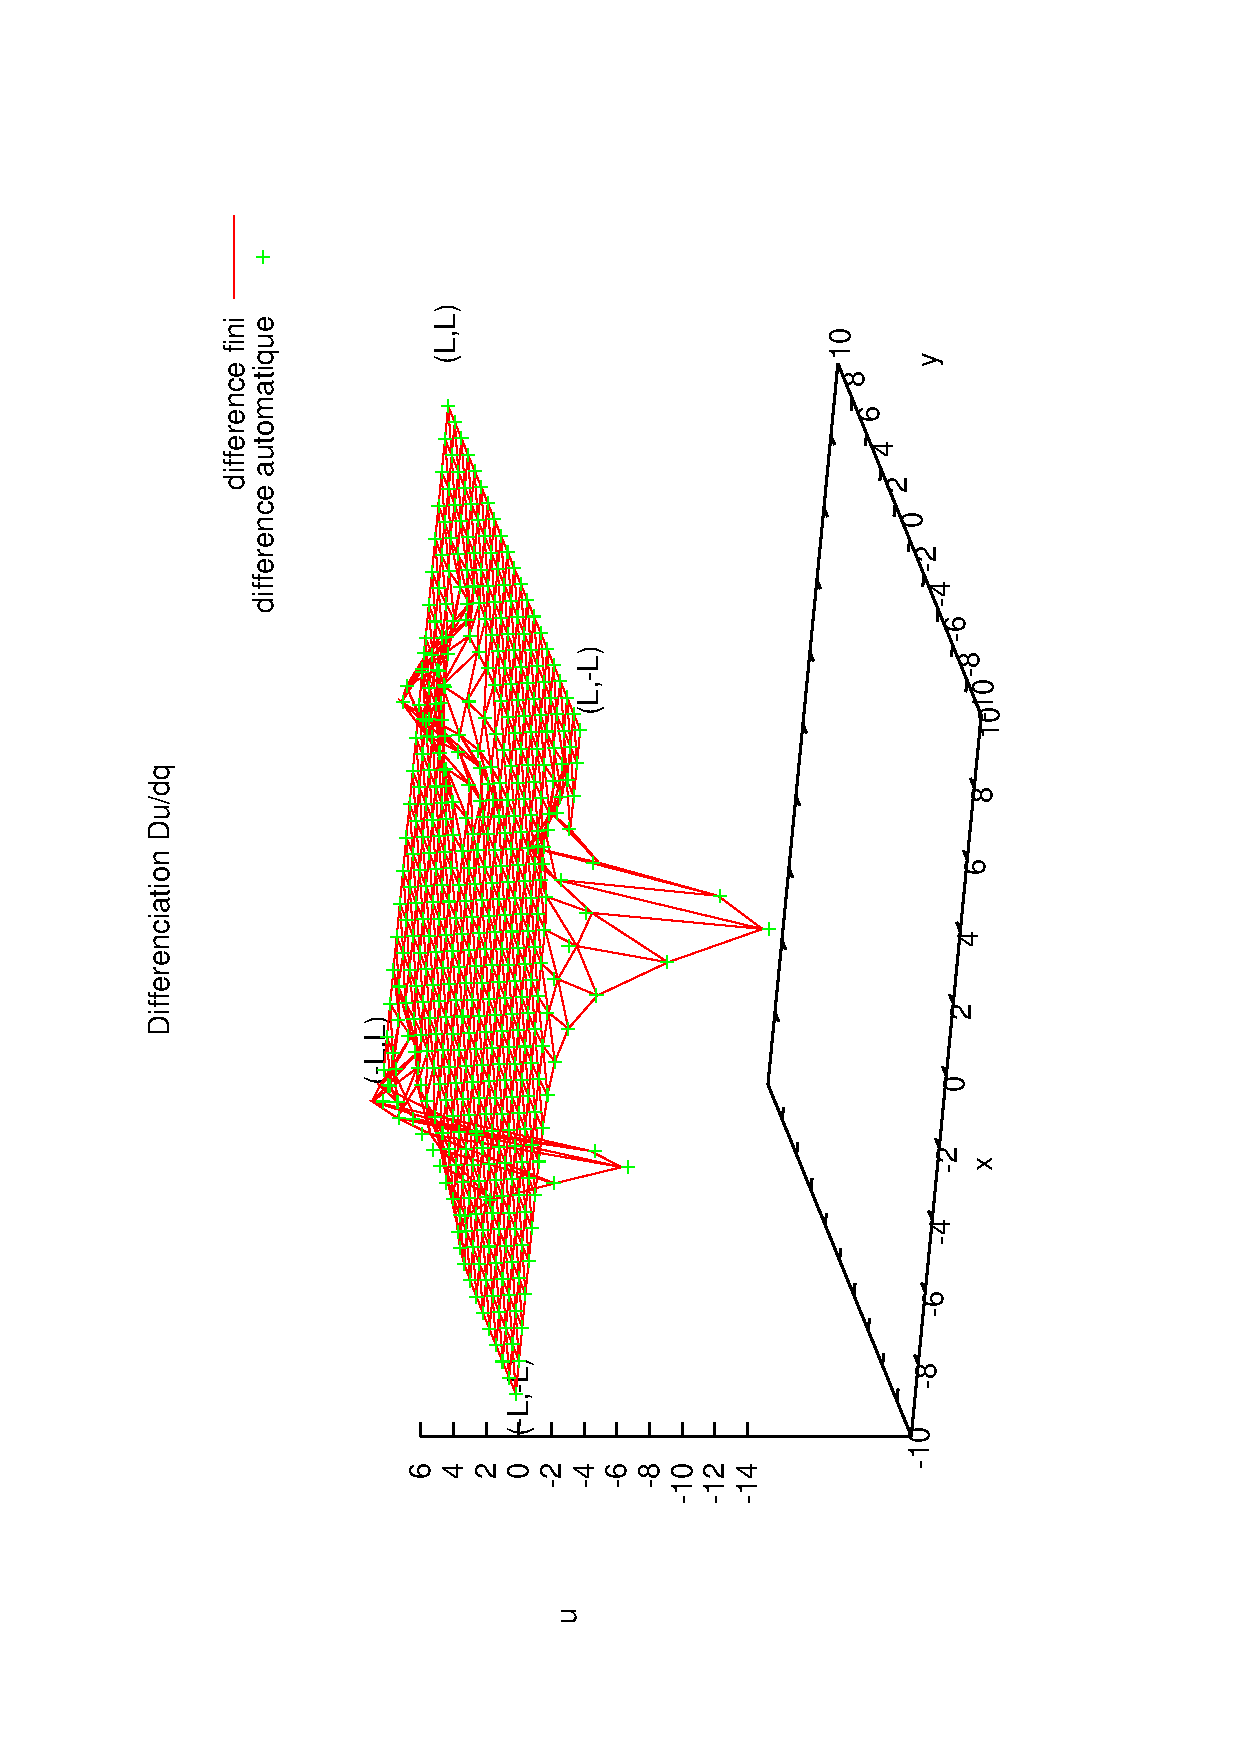
\includegraphics[ width=7cm, height=7cm,angle=-90]{DUdq}%
\end{center}
%%%%%%%%%%%%%%%%%%%%%%%%%%%%%%%%%%%%%%%%%%%%%%%%%%%%%%%%%%%%%%%%%%%%%%%%%%%%%%%%%%%%%%%%%
%=======================================================================================%
%%%%%%%%%%%%%%%%%%%%%%%%%%%%%%%%%%%%%%%%%%%%%%%%%%%%%%%%%%%%%%%%%%%%%%%%%%%%%%%%%%%%%%%%%
\section{Extention du problème en dimension 3}
%%%%%%%%%%%%%%%%%%%%%%%%%%%%%%%%%%%%%%%%%%%%%%%%%%%%%%%%%
\subsection{Schéma en dimension 3}
Quitte à exposer la partie modélisation et variationel, on rentre directement dans le schéma donné :
\[
\begin{split}
\frac{u^m_i-u^{m-1}_i}{\delta t} 
& -\frac{\sigma_1^2}2\frac{\partial^2 u^m_i}{\partial x^2}
  -\frac{\sigma_2^2}2\frac{\partial^2 u^m_i}{\partial y^2}
  -q\sigma_1\sigma_2\frac{\partial^2 u^m_i}{\partial x\partial y} \\
& +\mu_1\frac{\partial u^m_i}{\partial x}
  +\mu_2 \frac{\partial u^m_i}{\partial y}+r u^m_i  
  +i\frac{u^m_{i}-u^m_{i-1}}{{(M-m)\delta t}}=0 \\
& u^0_i(x,y)=(\frac{i\delta z}T -e^x-e^y)^+, \\
& u^m_I(x,y)=(\frac{I\delta z}T -e^x-e^y)^+~~~~\forall x,y,i,m
\end{split}
\]
Ce qui donne :
\[
\begin{split}
\frac{1}{\delta t} (u^m_i+i.\frac{u^m_i}{M-m})
& -\frac{\sigma_1^2}2\frac{\partial^2 u^m_i}{\partial x^2}
  -\frac{\sigma_2^2}2\frac{\partial^2 u^m_i}{\partial y^2}
  -q\sigma_1\sigma_2\frac{\partial^2 u^m_i}{\partial x\partial y} \\
& +\mu_1\frac{\partial u^m_i}{\partial x}
  +\mu_2 \frac{\partial u^m_i}{\partial y}+r u^m_i  
  =i.\frac{u^m_{i-1}}{{(M-m)\delta t}} + \frac{u^{m-1}_i}{\delta t}
\end{split}
\]
En comparant avec le schéma du cas dimension 2 :
\[
\begin{split}
\frac{1}{\delta t} (u^m)
& -\frac{\sigma_1^2}2\frac{\partial^2 u^m}{\partial x^2}
  -\frac{\sigma_2^2}2\frac{\partial^2 u^m}{\partial y^2}
  -q\sigma_1\sigma_2\frac{\partial^2 u^m}{\partial x\partial y} \\
& +\mu_1\frac{\partial u^m}{\partial x}
  +\mu_2 \frac{\partial u^m}{\partial y}+r u^m 
  =\frac{u^{m-1}}{\delta t}
\end{split}
\]
On peut alors résoudre le cas de dimension 3 en itérant plusieurs résolutions du cas de dimension 2, avec des petits changements des coefficients dans l'écriture matricielle de l'quation linéaire ~\eqref{schema2D-matriciel}  
%%%%%%%%%%%%%%%%%%%%%%%%%%%%%%%%%%%%%%%%%%%%%%%%%%%%%%%%%
\subsection{Iso-surface en dimension 3}
\begin{wrapfigure}{r}{0.5\textwidth}
  \begin{center}
    %\includegraphics[width=0.48\textwidth]{gull}
    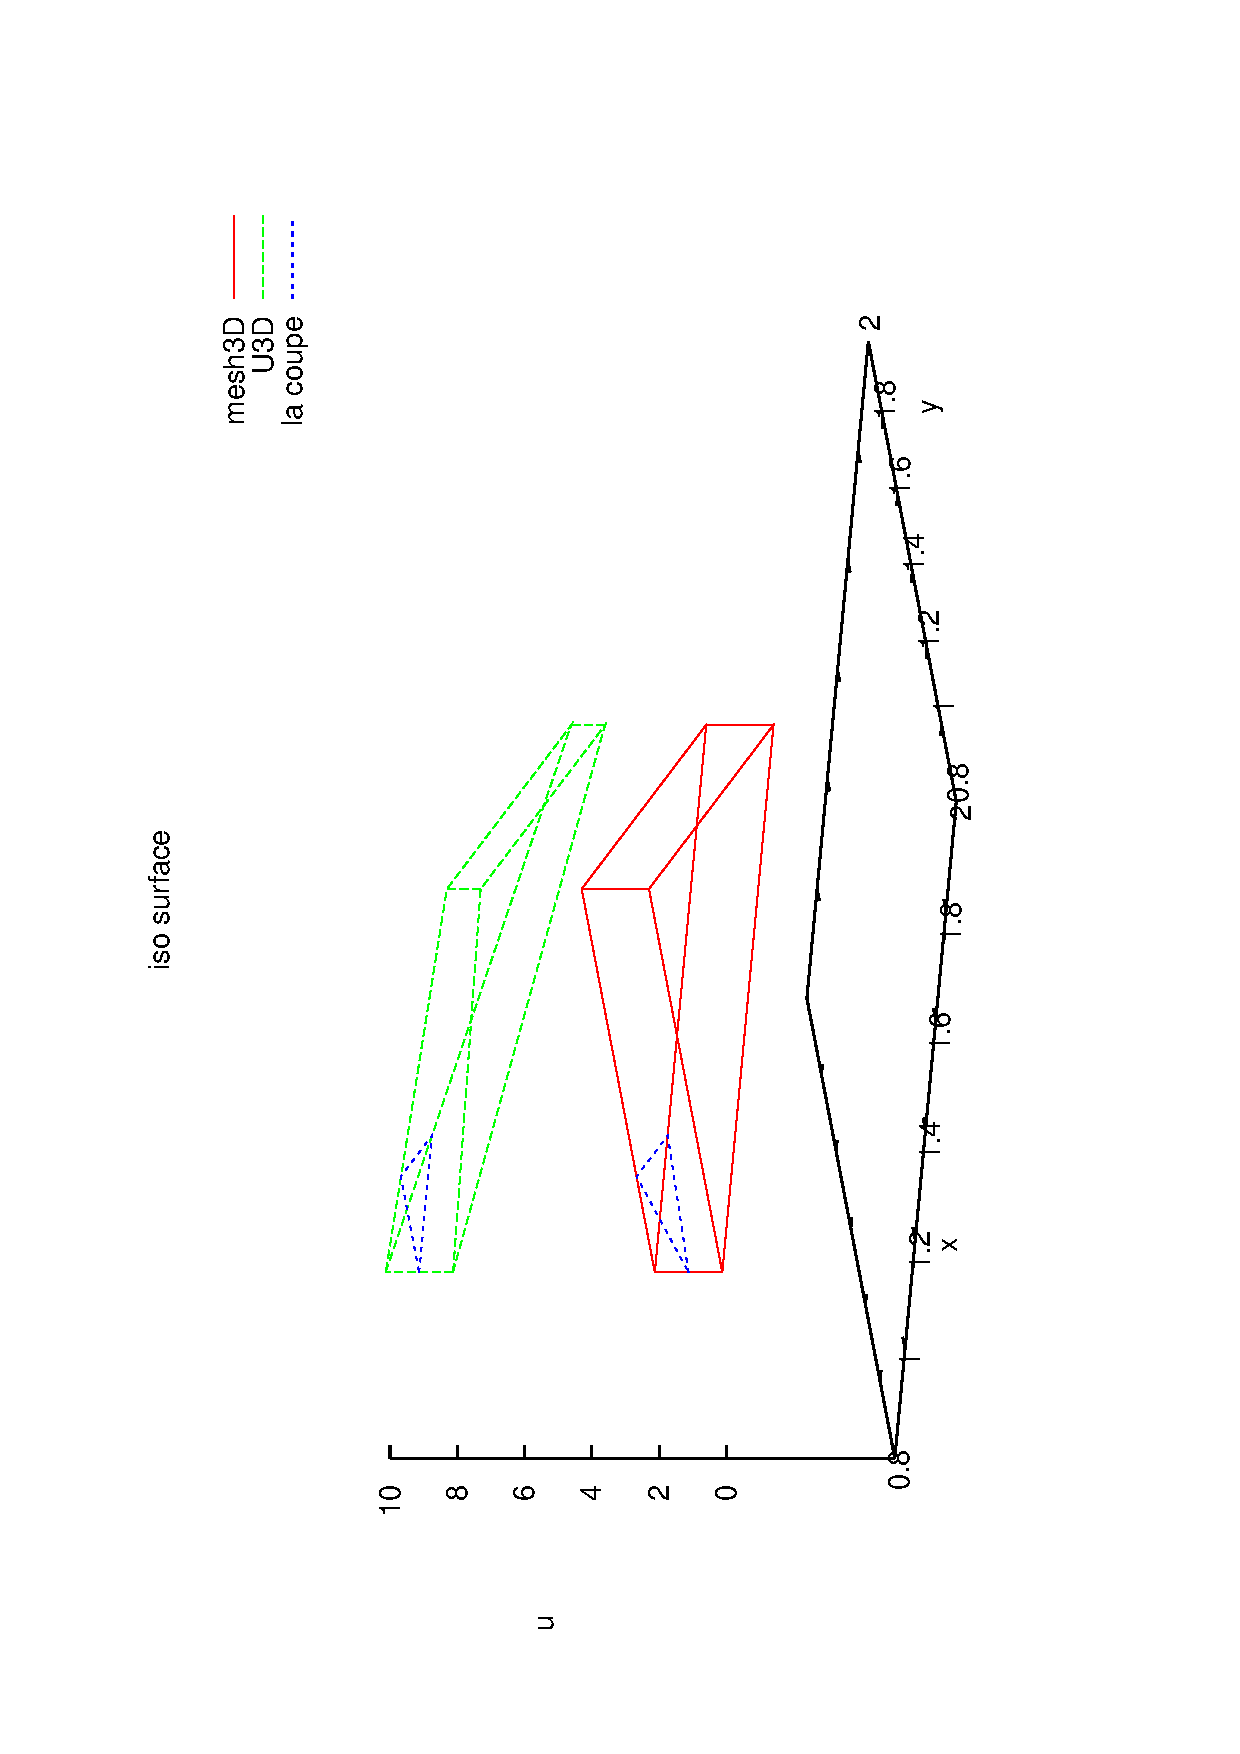
\includegraphics[angle=-90, scale=0.3]{iso-surface}
  \end{center}  
\end{wrapfigure}
%%ctntodo parpic package
Pour tracer une iso-surface de la solution en 3D, on se ramène dans le cas d'un un parallèlotope simple, construit sur un triangle et deux couches consécutifs de solution et de maillage. Une valeur donnée est considérée comme un plan qui coupe la fonction $u3D$ en certains points. En regardant la proportion des segments formés par ces points dans chaque côté du parallèlotope de $u$, on peut transformé cette proportion dans le parallèlotope correspondant du maillage. Il reste à associer à chaque iso-surface une couleur spécifique pour avoir enfin une visualisation visible. 
%%%%%%%%%%%%%%%%%%%%%%%%%%%%%%%%%%%%%%%%%%%%%%%%%%%%%%%%%
\subsection{Solution trouvée en dimension 3}
Quelques graphiques résultant des calculs de la solution asisan :
\begin{center}
 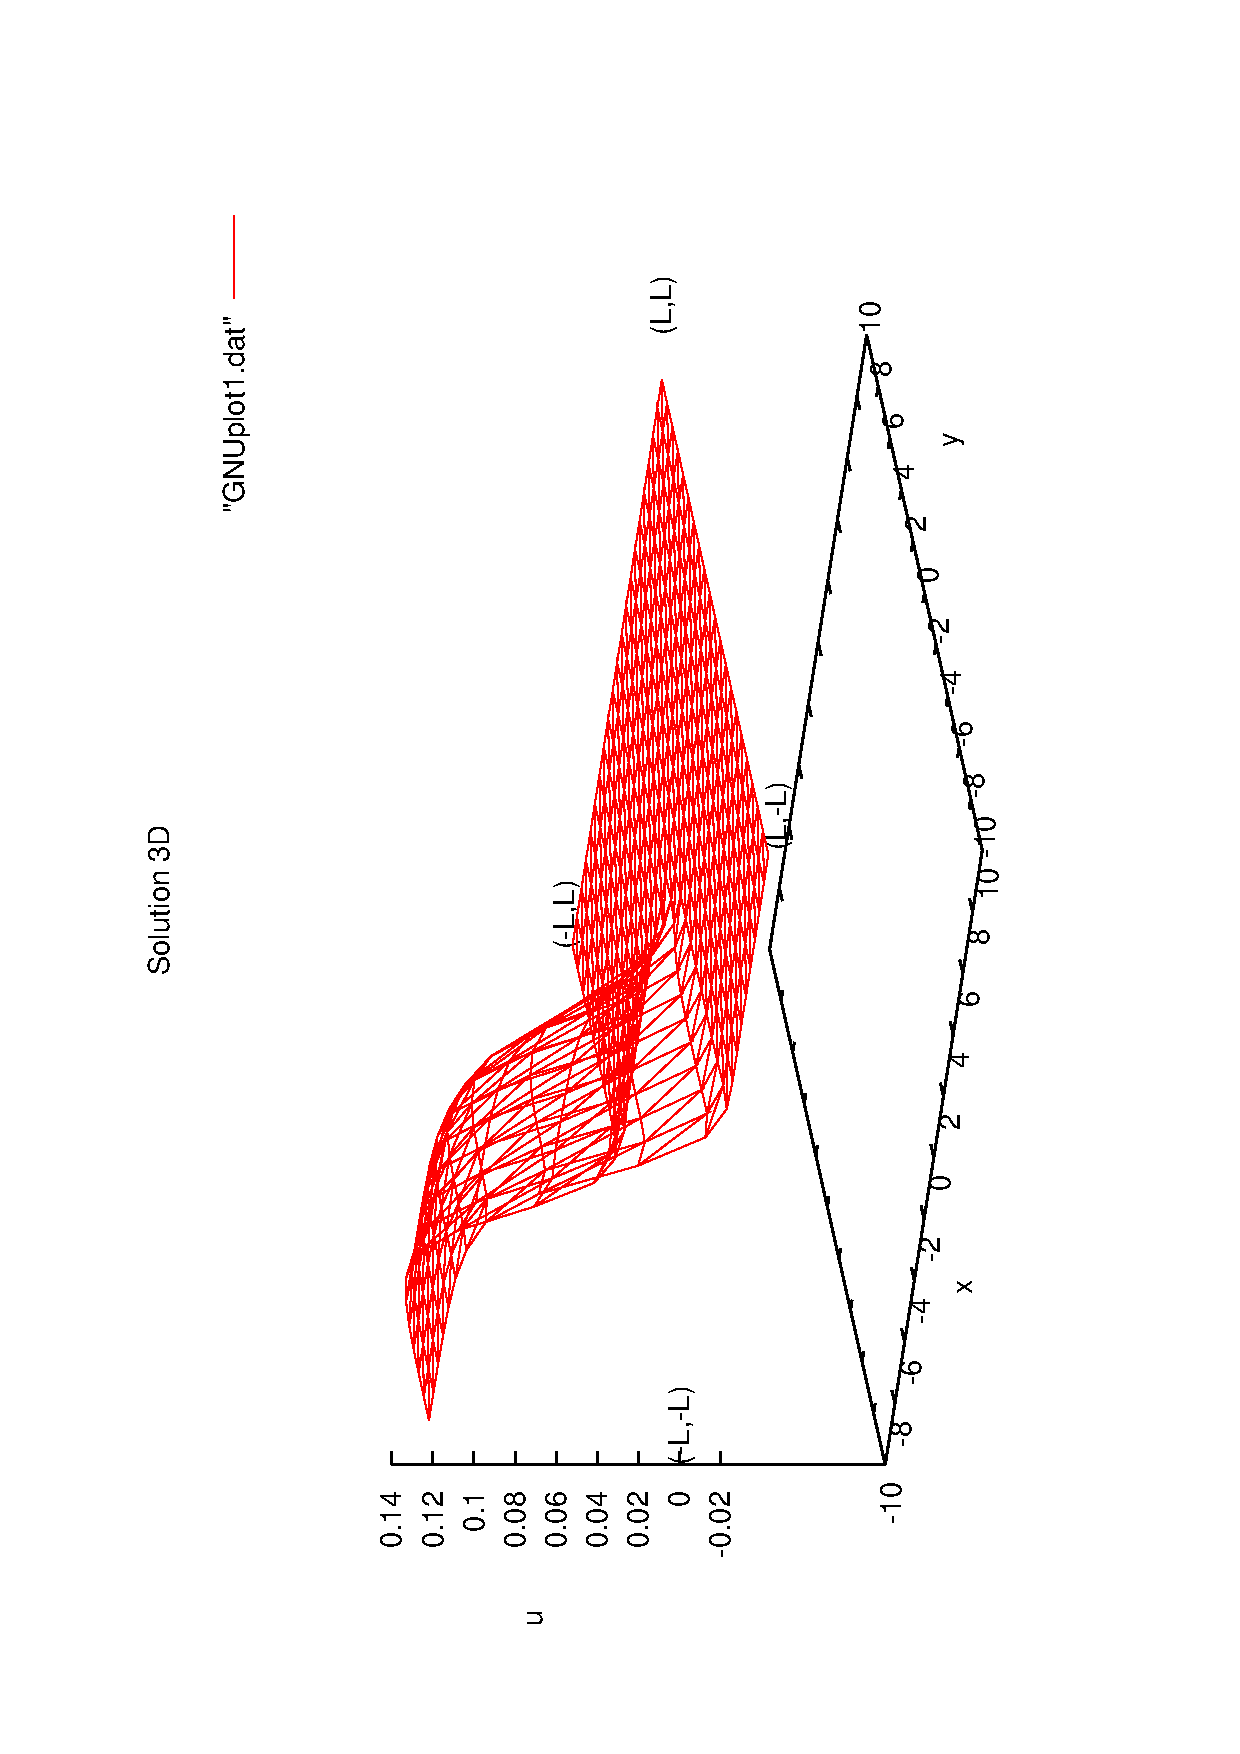
\includegraphics[ width=7cm, height=7cm]{Solasian}%
 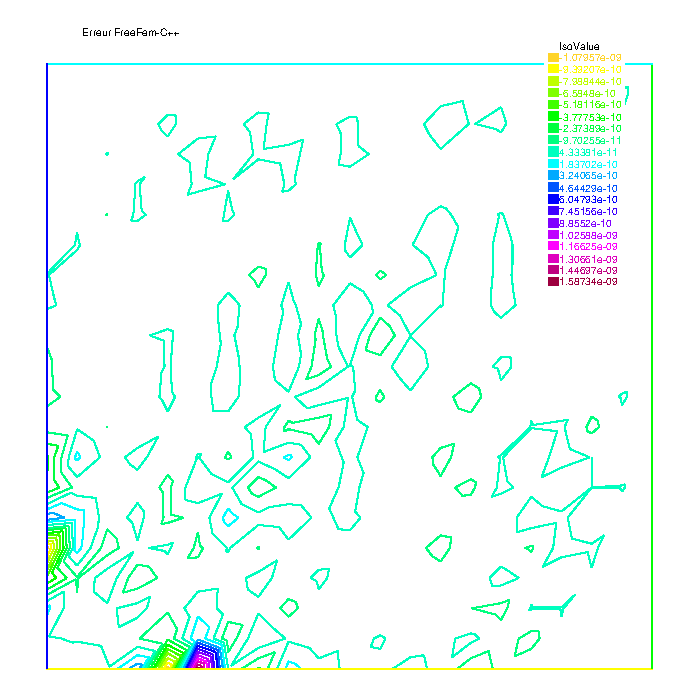
\includegraphics[ width=7cm, height=7cm]{Erreurasian}%
\end{center}
Les graphiques avec OpenGL :
\begin{center}
 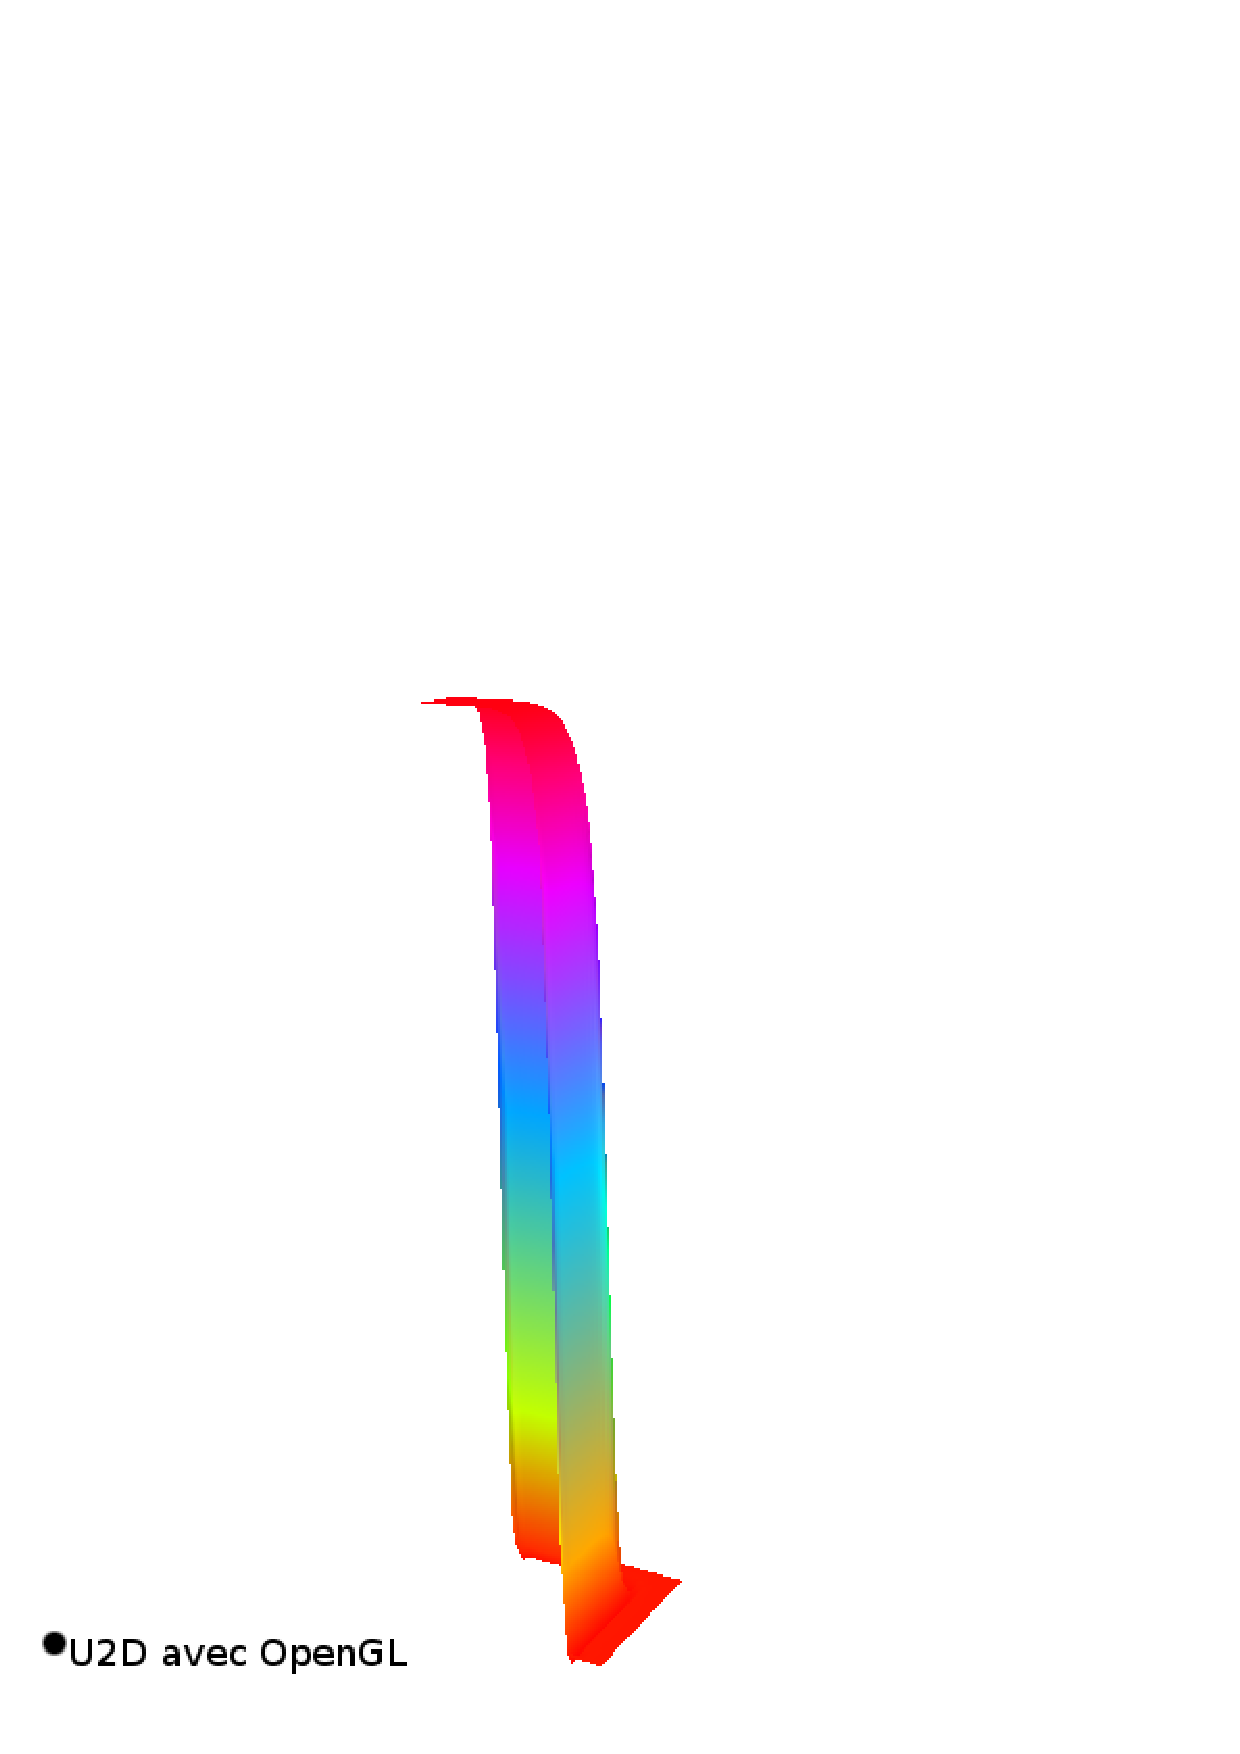
\includegraphics[ width=7cm, height=7cm]{U2D-OpenGL}%
 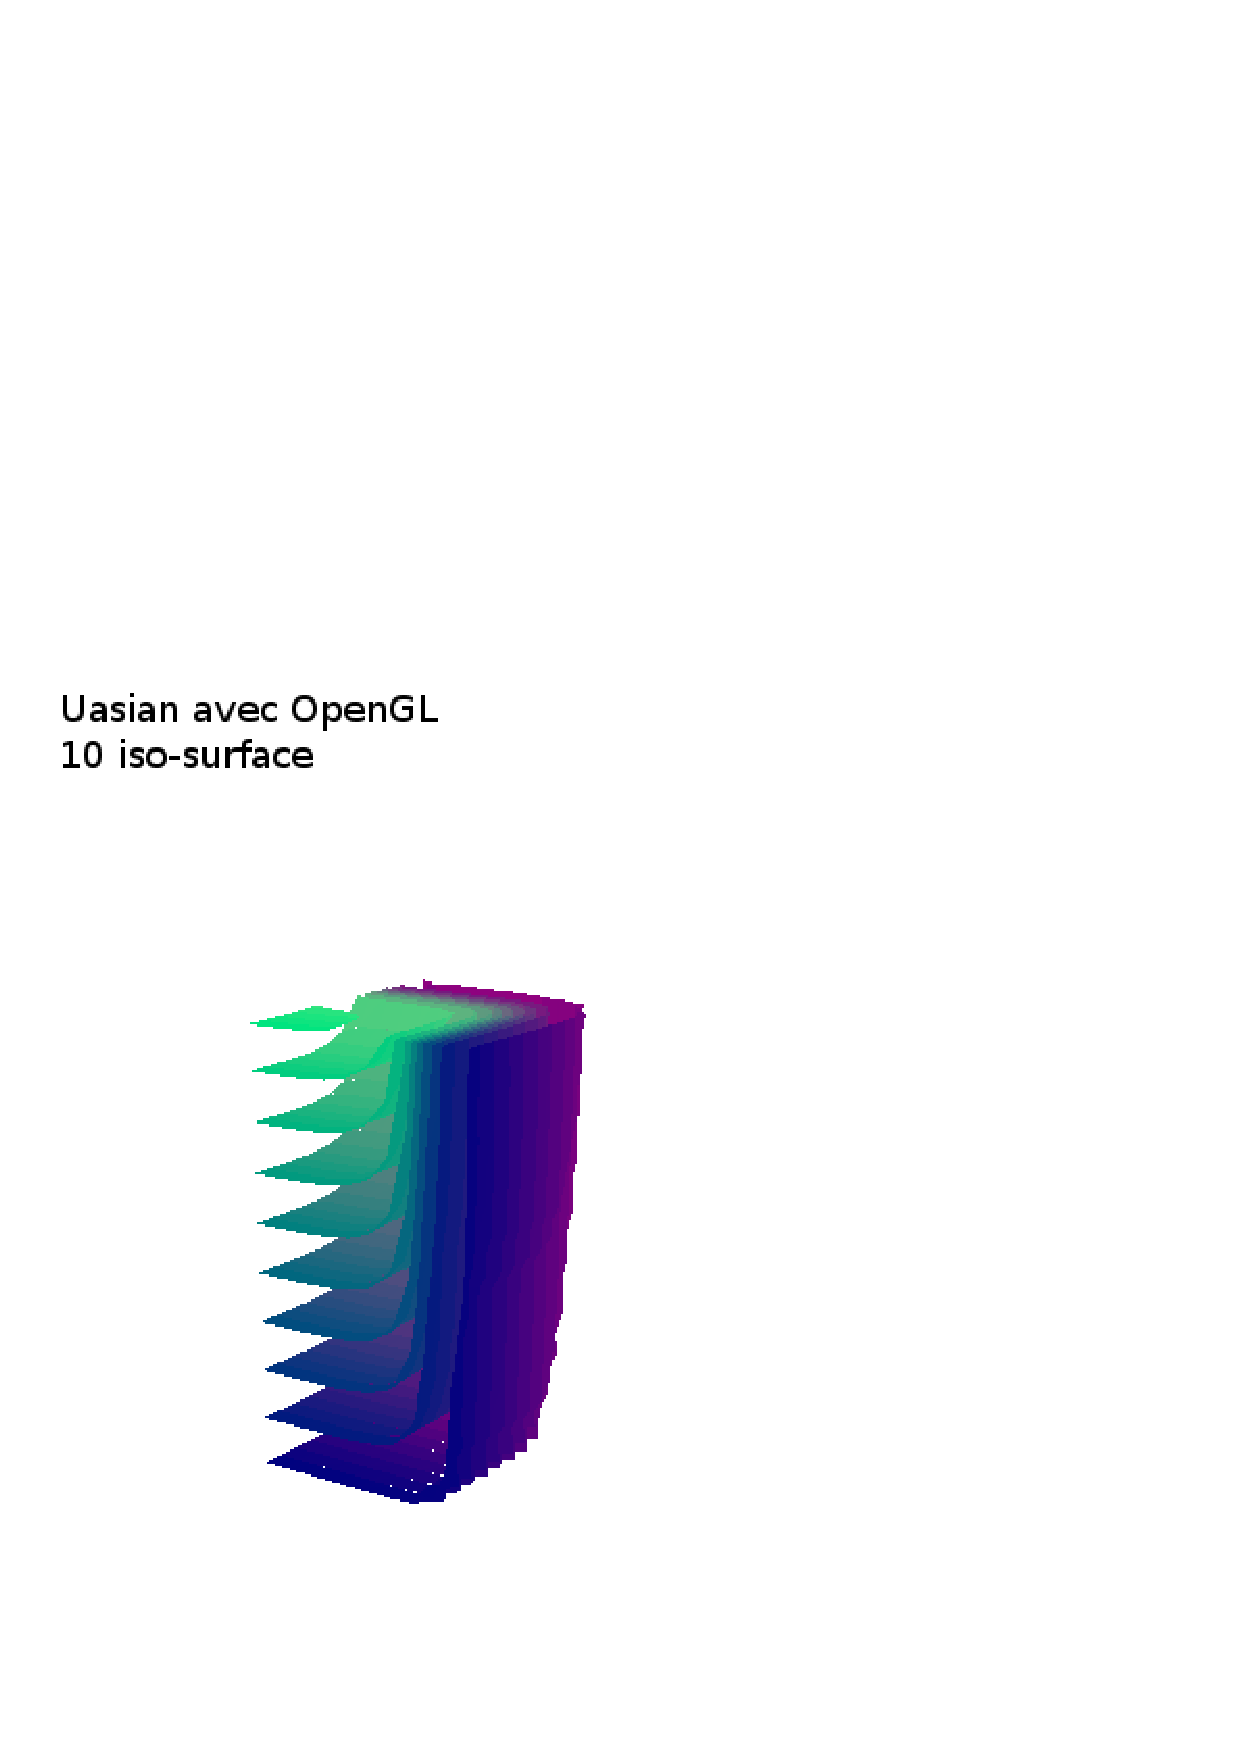
\includegraphics[ width=7cm, height=7cm]{Uasian-OpenGL}%
\end{center}


\vspace{10cm}
%%%%%%%%%%%%%%%%%%%%%%%%%%%%%%%%%%%%%%%%%%%%%%%%%%%%%%%%%%%%%%%%%%%%%%%%%%%%%%%%%%%%%%%%%
%=======================================================================================%
%%%%%%%%%%%%%%%%%%%%%%%%%%%%%%%%%%%%%%%%%%%%%%%%%%%%%%%%%%%%%%%%%%%%%%%%%%%%%%%%%%%%%%%%%
\section{Annexe}
%%%%%%%%%%%%%%%%%%%%%%%%%%%%%%%%%%%%%%%%%%%%%%%%%%%%%%%%%%%%%%%%%%%%%%%%%%%%%%%%%%%%%%%%%
%=======================================================================================%
%%%%%%%%%%%%%%%%%%%%%%%%%%%%%%%%%%%%%%%%%%%%%%%%%%%%%%%%%%%%%%%%%%%%%%%%%%%%%%%%%%%%%%%%%
\subsection{Programmation-Trucs et Astuces}
\begin{itemize}
\item Création d'un fichier Makefile facilite la compilation du programme.
\item Création des script de Gnuplot, qui permet la visualisation imédiate lors de l'exécution du programme, afin de voir le comportement des fonctions.
\item Utilisation de l'instruction de C :\\ 
	\hspace{2cm} system("commande shell"); \\Celle-ci peut exécuter le script de Gnuplot, gestion de fichier ....ect.. lors du lancement du programme.
\end{itemize}


%=================================Plan d'etude=======================================%
\begin{center}
\resizebox{6cm}{0.75cm}{\bsc{Plan d'étude}} \footnote{Explication du plan d'étude}
\end{center}
\vspace{2cm}
%===========================%
\begin{center}
\begin{pspicture}(-7,-5)(7,5)
%===
\rput(-2,5){\rnode{A}{\psframebox {\begin{tabular}{c}
										\large\textbf{Etude du}\\
										\large\textbf{phénomène}
									\end{tabular}}
		   }}
%===
\rput(-2,3){\rnode{B}{\psframebox{\huge E.D.P}}}
%===
\rput(7,5){\ovalnode{Bbis}{
							\begin{tabular}{c}
								\textbf{Résolution}\\
								\textbf{analytique}
							\end{tabular}}
			}
%===
\rput(-2,1){\rnode{C1}{\resizebox{6cm}{0.5cm}{\psframebox{%
							\begin{tabular}{c}
								\textbf{Résolution}\\
								\textbf{numérique}
							\end{tabular}}}
		    }}
%===
\rput(-2,-1){\rnode{C2}{\resizebox{8cm}{0.75cm}{\psframebox{%
							\begin{tabular}{c}
							\textbf{Analyse mathématique} \\
							    \psframebox{Existance et unicité}
							    \psframebox{Discrétisation} 
								\psframebox{Méthode à appliquer}			
							\end{tabular}}}
		    }}
%===
\rput(-2,-3){\rnode{C3}{\resizebox{10cm}{0.75cm}{\psframebox{%
							\begin{tabular}{c}
							\textbf{Modèle informatique} \\
							    \rnode{C31}{\psframebox{Données d'entrée}} \hspace{1cm}
							    \rnode{C32}{\psframebox{Programme}} \hspace{1cm}
								\rnode{C33}{\psframebox{Données de sortie}}			
							\end{tabular}}}
		    }}
\ncline{->}{C31}{C32}\par
\ncline{->}{C32}{C33}\par
%===
\rput(7,-0.5){\rnode{Se}{\psshadowbox {\begin{tabular}{c}
										\textbf{Solution}\\
										\textbf{analytique}
									\end{tabular}}}}
%===
\rput(7,-2){\rnode{Sn}{\psshadowbox {\begin{tabular}{c}
										\textbf{Solution}\\
										\textbf{numérique}
									\end{tabular}}}}



\ncdiag[angleA=0, angleB=-90, arm=.5, linearc=.2]{B}{Bbis}
\ncline{A}{B}\par
\ncline{B}{C1}\par
\ncline{C1}{C2}\par
\ncline{C2}{C3}\par
\ncline{->}{Bbis}{Se}\par
\ncbar[angle=-180]{->}{A}{C31}
\ncbar[angle=0]{->}{C33}{Sn}
\end{pspicture}
\end{center}
%===============PLAN D'ÉTUDE=================================================%


\end{document}